\documentclass{ucl_thesis}

%twoside for double page printing
\usepackage{graphics}
\usepackage{graphicx}
\usepackage{color}
\usepackage{verbatim}
\usepackage{algorithm}
\usepackage{algorithmic}
\newcommand{\theHalgorithm}{\arabic{algorithm}}
\usepackage[square]{natbib}

\usepackage[font=footnotesize,labelfont=bf,singlelinecheck=on]{caption}
\usepackage[hyphens]{url}

\usepackage{amsmath}
% Uncomment this to activate the TikZ library, which is useful for fancy block-diagrams.
%    \usepackage{tikz}
%    \usetikzlibrary{positioning,arrows,shapes.misc}
\usepackage{multirow}

%\numberwithin{algorithm}{chapter}
%\usepackage{epsf}
\usepackage{fancyvrb}

%\documentclass[12pt,a4paper]{article}
%\usepackage[utf8]{inputenc}
\usepackage[english]{babel}
%\usepackage{amsmath}
%\usepackage{amsfonts}
%\usepackage{amssymb}
%\usepackage{graphicx}
%usepackage[left=2cm,right=2cm,top=2cm,bottom=2cm]{geometry}
%
%\usepackage[]{natbib}

% // TODO: add pagenumbers

%% LISTINGS
\usepackage{color}
\usepackage{listings}
\definecolor{mygreen}{rgb}{0,0.6,0}
\definecolor{mygray}{rgb}{0.5,0.5,0.5}
\definecolor{mymauve}{rgb}{0.58,0,0.82}
\definecolor{purple}{rgb}{0.28,0.23,0.5}
\lstdefinestyle{customcpp}{
  belowcaptionskip=1\baselineskip,
  breaklines=true,
  frame=L,
  xleftmargin=\parindent,
  language=C++,
  showstringspaces=false,
  basicstyle=\footnotesize\ttfamily,
  keywordstyle=\bfseries\color{green},
  commentstyle=\itshape\color{purple},
  identifierstyle=\color{blue},
  stringstyle=\color{orange},
  numbers        = left,
  stepnumber     = 5,
}
%%

%% figure template
\newcommand{\myfig}[6]{%
\begin{figure}[h!]\centering%
	\begin{minipage}[b]{0.49\linewidth}\centering%
		\includegraphics[width=\textwidth]{#2}%
		\caption{#3}%
		\label{fig:#1}%
	\end{minipage}%
	\begin{minipage}[b]{0.49\linewidth}\centering%
		\includegraphics[width=\textwidth]{#5}%
		\caption{#6}%
		\label{fig:#4}%
	\end{minipage}%
\end{figure}%
}
%%

%% shortcuts
%Malcolm added some custom commands here - you can make your own!
\newcommand{\vect}[1]{\boldsymbol{#1}}
\newcommand{\figref}[1]{(Fig. \ref{#1})}
\newcommand{\secref}[1]{(Section \ref{#1})}
\newcommand{\chpref}[1]{(Chapter \ref{#1})}
\def\etal{{et~al.}}
\def\ie{{\it i.e.,\ }}
\def\etc{{\it etc.,\ }}
\def\eg{{\it e.g.,\ }}
\def\vs{{\it vs.\ }}
\newcommand{\mytilde}{\raise.17ex\hbox{$\scriptstyle\mathtt{\sim}$}}
%%

\author{Aron Monszpart}
\title{Hand-held Scanning of Surface Details}
\def \supervisor {Dr. Gabriel Brostow}
\date{September 2013}

\begin{document}

\bibliographystyle{plainnat}
\maketitle
\numberwithin{algorithm}{chapter}
\setcounter{page}{1}
\pagenumbering{roman}
\pagestyle{plain}

% Notice how the star "*" is used throughout LaTex to modify the normal behavior. For example, \section* instead of \section 
% tells LaTex NOT to number this section.


\newpage
\section*{Abstract}

The accurate acquisition of fine detailed 3D geometry using a hand-held scanning device is an exciting research topic providing space for innovation. Current state-of-the art reconstruction systems are more focused on large-scale environments and real-time operation than surface details. Investigation is to be conducted to identify the reasons for the over-smoothed nature of the output from modern multi-view stereo and structured lighting solutions. Using the results a proposal to a system can be made, that will make use of recent achievements in the field of machine vision. By applying non-linear filtering using input from multiple sensors great increase in accuracy is expected. Surfaces will be recorded from very close distance to capture as many details as possible. The usage of motion sensor information will solve problems of localisation emerging in these less textured environments.


\newpage
\section*{Acknowledgements}
First and foremost I offer my sincerest gratitude to my supervisor, Dr. Gabriel Brostow, who has not spared time, connections or resources to support and guide the success of our project. I would also like to thank Dr. Neill Campbell for his continuous help and support regarding theoretical and practical advice as well computational resources. I would like to acknowledge Dr. Oisin Mac Aodha for his continuous feedback and advice steering the course of our project. In addition, I am very grateful for all the help and advice I have received from Fabrizio Pece, Malcolm Reynolds, Clement Godard, Peter Rennert, the whole PRISM group at University College London and everyone else, who has supported me during the accomplishment of the project.

%\setcounter{tocdepth}{2}
\tableofcontents
\listoffigures
%\listoftables
%\listofalgorithms
\newpage

\setcounter{page}{1}
\pagenumbering{arabic}
\pagestyle{plain}

\chapter{Introduction and Background} 

The possibility to develop a flexible, easy to use, relatively environment independent hand-held acquisition process is to be discovered in the frames of this project. Hand-held 3D scanning is the process of acquiring measurements of real world objects and also of recording of accurate depth information about the surfaces of objects in a scene. A high quality measurement allows estimations to be executed on the acquired model yielding results validly transferable to the real world object. We define fine surface details to be the high frequency characteristics of surfaces that are visible to the sensor, but might get lost during the recording process. There exists technology (laser scanners \cite{DiebelThrun05} \cite{Schuon09}, photometric stereo \cite{Nehab05}) that allows these details to be extracted, but the applications require special circumstances and a highly controlled environment. Other solutions, as Kinect Fusion \cite{Izadi11} produce robust and even real-time 3D reconstructions of scenes but fail to pay attention to the retrieval of fine surface details. \\

\par In this project we targeted the acquisition of such fine surface details with any method that allows higher flexibility with regard to the required environment. We started our investigation by evaluating the applicability of recent achievements of the fields multi-view stereo, active stereo and dense 3D reconstruction. 
\par The results of the 3D reconstruction process are used in a large variety of fields influencing many aspects of our lives. The scanning method usually used is simultaneously determined by the level of need for quality and the possibilities in the given acquisition environment. We will illustrate the wide usage of geometry acquisition and the space for a possible improvement on cost, system size and accuracy by a couple of usage examples.

3D scanning is widely used in the field of medicine in many forms. Amongst others it is used for body scanning to discover body structure related problems and to monitor effectivity of treatment \cite{photomodeler_biology}. The work of surgeons can be assisted by combining the powers of augmented reality and accurate, online 3D scanning. IEEE Spectrum \cite{Spectrum_IEEE} reported about a project in March 2013, where the work of Ben Glockner \cite{ben_glockner} and his group at Microsoft Research used Kinect Fusion \cite{Kinect_fusion} to create a live 3D model of a patient's skull. This model was then used to re-project useful information for the surgeon to the "scene", the patient's head on the operating table.
\par 3D printing has become a rapidly growing entertainment industry. A good demonstration of the potential lying in an easily operated 3D scanner is the online 3D model repository, {\it Makerbot.com}'s desktop table scanner prototype Makerbot Digitizer \cite{Digitizer} introduced on the SXSW 2013 conference \cite{SXSW}.
\par Accurate 3D scanning is also very important in the field of cultural heritage preservation \cite{Michelangelo_Project}. Results acquired here or at other venues of scanning can be used to replicate real world models for educational purposes as well. Companies in the manufacturing industry can list several dozens of use cases for accurate 3D scanning \cite{Creaform3D}. 
\par With respect to \cite{photomodeler_biology} the previously mentioned use cases all operate with scanners based on 3D technology. There exists hand-held laser scanners \cite{Creaform3D}, but their price and physical dimensions leave room for improvement. In the fields of crime scene forensics and the film and animation industry, there is precedence for application of high resolution digital camera images for 3D reconstruction \cite{Photomodeler_film} \cite{Photomodeler_forensics}. The usage of the software requires high cost digital cameras, manual calibration and advanced knowledge to achieve the high quality results demonstrated on the product page. 
\par During the planning of the project the system's applicability in the film industry as example target was emphasized. Low-budget or amateur films using small-scale models of the real world usually apply a severe amount of post processing to the footage. Having an exact, high resolution 3D model of the scene set would enable them to increase the quality of currently applied special effects and extend their palette of tools intensely. Particle systems have a very wide field of applicability in this context, and providing the physics simulator with highly accurate 3D data is essential to high quality animations.\\

\par The presented use cases show, that there lies a strong commercial perspective in a cheap, easy to use and highly accurate hand-held 3D scanning solution. In \chpref{chp:related_work} the scientific potential of such a project is demonstrated. In \chpref{chp:my_system} we present the concept of our approach, in \chpref{chp:validation} we present the evaluation of the developed solutions to then assess our experiences in \chpref{chp:discussion}.

%%% ------------------ Background ------------------ %%%

\par The targeted system attempts to solve the problem of 3D reconstruction of fine surface details in static scenes. We have seen various examples of sparse 3D reconstruction methods using the achievements of multi-view stereo, structure from motion and SLAM techniques. In recent years, a large leap has been made in dense 3D reconstruction by RGB-D based methods. By designing this system we attempted to address inaccuracies produced by the above mentioned methods to refine high frequency details in small segments of the reconstructed models. The system designed acknowledges the power of SLAM performed on the dense model incorporated in the areas of RGB-D based methods. We also recognize the power of other research areas, where inter-sensory information is used to enhance output quality. 
\par We claim the hypothesis that there is data collected by the capturing system but is discarded early in the reconstruction pipeline of a standard 3D reconstruction system. We looked for methods that enable this information to be reintegrated into the results of the reconstruction. The solution was designed based on the alleged potential of iterative, cost-volume based joint bilateral filtering with sub-pixel accuracy published by \citep{cvpr-07-qingxiong-yang}.

Since two baseline methods, RGB and RGB-D, are targeted for improvement and each of them involve a different tree of densely branched research areas, many concepts were visited for the following reasons. To exactly discover the space for innovation, to consider the transferability of well working solutions as algorithmic building blocks to areas of critical need of better performance and to stimulate the creation of novel combinations of methods. The science of dense 3D reconstruction from RGB-D data was researched the most, since the performance of this field was found to yield higher quality initial results than the areas of multi-view stereo. Active stereo solutions were needed to support our hypothesis, that a solution based on recent results in smooth 3D reconstruction and earlier results in depth up-sampling using the iterative, cost-volume based joint bilateral filter by \cite{cvpr-07-qingxiong-yang} will allow high frequency details to be added to the reconstructed model from any new viewpoint, that's pose can be estimated.

%%% CHAPTER RELATED WORK %%%
\chapter{Related work} 
\label{chp:related_work}

\par The three major fields we were interested in during researching existing methods were multi-view stereo and structure from motion, dense 3D reconstruction using active lighting and depth up-sampling. Auxiliary methods necessary to design and build the combined pipeline using the achievements of the methods serving as basis for our hypothesis were explored, namely camera calibration and feature detection.

\section{Stereo correspondence}
With the evolution of stereo imaging three major works review the state-of-the art techniques among dense two-view stereo correspondence algorithms \cite{ScharsteinS02}, and among multi-view stereo reconstruction algorithms \cite{Seitz:2006}, \cite{Strecha:2008}. The taxonomies defined aid the analysis of current state-of-the art algorithms and will therefore be introduced in more detail in the following paragraphs.

\subsection{Dense two-view stereo correspondence} 
\label{subsub:densestereo}

\par The results presented in the first work have had a significant impact on the machine vision community by providing test datasets for two-view stereo used for evaluation even very recently \cite{Yang12} \cite{MacAodhaDepthSuperResECCV2012}. 
\par Concepts as representation, rectification and disparity space get defined as common terms used by stereo matching algorithms. Although the work focuses on uni-valued disparity functions it groups multi-view techniques into multi-valued, voxel-based and layer-based categories based on their representations of internal states and output. It also mentions deformable models, triangulated meshes and level-set methods as alternative approaches.
\par A taxonomy of stereo matching algorithms is introduced giving an overview of the most important steps of a stereo matching approach. These are {\it matching cost computation}, {\it cost aggregation}, {\it disparity computation} and {\it disparity refinement}.
\par The most basic measures for {\it matching cost computation} are identified as squared intensity differences (SD), absolute intensity differences (AD), mean-squared error (MSE) and mean absolute difference (MAD). A large overview of more complex measures is given mentioning gradient-based measures, a sampling independent measure and iterative diffusion. SSSD and SSAD are measures mentioned as extensible to multiple baseline approaches.
\par {\it Cost aggregation methods} are grouped into two- and three-dimensional methods. The latter allows support for slanted surfaces. Solutions for {\it disparity computation and optimization} are grouped into local methods, global optimization, dynamic programming and cooperative algorithms. 
\par {\it Disparity refinement} will be an area of emphasis in our approach. Areas of continuous optimization are mentioned to be less common (the usage of optic flow or splines) compared to discrete methods targeting sub-pixel disparity estimates. Iterative gradient descent, curve fitting, median filtering and propagation over neighbourhood are the mentioned techniques in the paper. Our approach will most likely build on disparity refinement by bilateral filtering introduced in \cite{cvpr-07-qingxiong-yang}.

\subsection{Multi-view stereo reconstruction}

Our targeted research will attempt to rely on the performance of multi-view stereo techniques. Therefore it is important to have an overview of the most relevant and recent solutions in the field. The work in \cite{Seitz:2006} continues on the path of the previously discussed taxonomy referenced in Section \ref{subsub:densestereo}. The aspects investigated in the paper are {\it scene representation}, {\it photoconsistency measure}, {\it visibility model}, \textit{shape prior}, \textit{reconstruction algorithm}, and {\it initialization requirements}.

\par In terms of {\it scene representation} the main methods of the algorithms reviewed are similar to the previous taxonomy: voxel-based, level-sets, polygon meshes and multiple disparity maps. Whilst voxel-grids are easier to implement, the resolution as parameter can have a large impact on the results (an adaptive oct-tree representation is a common solution to this problem \cite{jevans1989adaptive}, as implemented in the Point Cloud Library \cite{PCL}.) Polygon meshes are stated to be very popular due to the fact, that they favour visibility computations. Indeed, one of the current state-of-the art techniques, \cite{FurukawaCSS10} rely heavily on visibility calculations to select the most relevant points of interest in large datasets. Another modern technique \cite{Tola12} uses multiple depth maps to escape the restrictions of a volumetric sampling grid.

\par {\it Photo-consistency measure} rates the state of the current reconstruction by its agreement with a set of input images as described in the paper. It gets grouped into methods operating in scene space and image space. In scene space the re-projection of a geometric entity (i.e. point) is evaluated by a selected error metric, as variance, sum of squared differences or normalized cross-correlation. In image space pixel intensity consistency is measured by warping images onto other images in the input set based on the supposed geometry model. This results in a term usually named prediction error. The former method is prone to volume shrinking due to the integration of error measures preferring smaller surfaces, whilst the latter method takes region of interest into account by emphasizing visible features of the geometry by integration of error over the set of input images. Our conclusion predicts that this can favour local accuracy in visible regions, but for higher genus objects, the completeness measure will probably suffer.

\par The {\it visibility model} is the third aspect of investigation regarding multi-view stereo algorithms according to the paper. Its purpose is to select images, cameras and pixels that contribute to the error metrics presented in the previous paragraph. In the review the models get classified into geometric, quasi-geometric and outlier-based approaches. The key question is which intensity disagreement should be taken into account when re-estimating the geometry. Geometric estimate visibility based on pixels or patches as done in \cite{FurukawaP07}. Quasi-geometric methods relief the computational load of large datasets by approximating visibility by clustering cameras, i.e. as its further developed upon in \cite{FurukawaCSS10}. Outlier based methods don't calculate visibility, but use measures from statistics to handle severe disagreement scores.

\par Especially interesting to our approach are the questions around {\it shape priors} since their role increases with low textured regions. Many methods operate using optimizations targeting minimal surfaces. According to the paper, scene based photo-consistency approaches and min-cut based solutions also suffer from problems of shrinking of the volume and smoothing of high curvature details. Furthermore, solutions seeking maximal surfaces usually operate based on voxel colouring and scene carving targeting the creation of the "largest photo-consistent scene reconstruction" named the "Photo Hull". A modification to this approach was later suggested, called "Photo Flux" \cite{boykov2006photohulls}. Maximal surface methods are stated to be good at high frequency details but produce errors in low texture regions. Local smoothness favouring methods attempt to solve this by using Markov Random Fields with surface based priors. The cross bilateral filtering technique in \cite{cvpr-07-qingxiong-yang} can be treated as an extension to the unary and pairwise costs of such an MRF.

\par In terms of {\it reconstruction algorithm} the paper assembles cost-function based approaches, iteratively evolving methods, depth-map merging solutions and surface fitting methods. The presented algorithms either contain {\it initialization requirements} about the size of the scene volume or a maximum disparity dynamic range.

\subsection{State-of-the art sparse multi-view stereo}

The basis of the emergence of successful dense multi-view stereo was partially built by powerful and robust camera pose estimation pipelines. Two major and in their methodology closely related pipelines were discovered during research. 
\par The Bundler \cite{SnavelySS06} system aligns multiple images containing parts of a larger scene to a consistent set of camera poses producing a sparse point cloud. In \cite{SNAVELY-IJCV08} the work is continued to enable internet-scale reconstruction. They use EXIF data from the images for initialization and to determine absolute location, SIFT key-points \cite{Lowe04} to align input images by estimating their relative locations and RANSAC \cite{fischler1981random} to calculate fundamental matrices based on image pairs. They then construct tracks of aligned image pairs being the output of their pose estimation algorithm. 
In \cite{AgarwalFSSCSS11} ("Building Rome in a day") further development is outlined to increase the performance of the reconstruction pipeline to be able to handle even larger sets of input data. The parallelisation possibilities of the pipeline are evaluated. In \cite{Tuite:2011:PTE:1978942.1979146}  ("PhotoCity") large-scale environment reconstruction is attempted to be made crowd-sourced using the tools of gamification. The product Microsoft Photosynth \cite{Photosynth} offers the capabilities of the developed pipeline powered by cloud-computing to provide an appealing photo-collection viewer. \\

\par A very popular pipeline the scientific community often uses is Visual Structure from Motion (VSFM). It uses the parallelised extraction algorithm of SIFT feature points SiftGPU \cite{siftgpu07wu}. The feature points are then registered over the sets of images to estimate their camera poses by minimising the reprojection error. The theory is based on the large-scale bundle adjustment technique \cite{agarwal2010bundle} implemented in parallel in Multicore Bundle Adjustment published in \cite{CWu11}. The project includes the later detailed CMVS \cite{FurukawaCSS10} algorithm to perform a dense reconstruction. The results of further research are most likely included in Google's MapsGL project \cite{MGL}.

\subsection{State-of-the art dense multi-view stereo} 
\label{sotadense}

In \cite{Strecha:2008} published benchmarking datasets for the comparison of multi-view stereo algorithms. A much slower but significantly more accurate acquisition process using a LIDAR time-of-flight scanner was applied, and error measures were defined appropriately. In their work, besides their own earlier algorithms \cite{strecha2004wide} \cite{strecha2006combined} the work published as \cite{FurukawaP07} called "Patch-based multi-view stereo" (PMVS) was treated as state-of-the art. They integrated modern techniques at the time including selection of robust features, iterative expansion of included images and filtering based on effective visibility constraints.

\par At this point of the science, the biggest question was how to handle the incredibly large amounts of input data meaning that photo-consistency measures and visibility checks had to be calculated over very large point sets of possibly corresponding points. These problems were addressed in \cite{agarwal2010bundle} and \cite{AgarwalFSSCSS11} as described earlier.

\par PMVS was later improved upon in \cite{FurukawaCSS10} titled "Clustering Views for Multi-view Stereo" (CMVS) allowing mega-scale image datasets to be used for large-scale reconstruction. This is achieved by introducing a local clustering of camera viewpoints to reduce the computational cost of photo-consistency calculations over the whole input image set.

\par \cite{Jancosek:2011} improved on the CMVS technique by introducing the term weakly supported surfaces denoting geometry with a lower coverage of robust, multi-view consistent feature points. This is done by including highly supported free space into the cost structure of the Markov Random Field construction.

\par In \cite{HHVu:2011} the theoretical foundations assessed in \cite{faugeras2002variational} (geometry processing methods including variational principles, surface evolution, partial differential equations, level set methods) were used to claim improvement towards the PMVS technique. Although large-scale reconstruction is targeted, a higher level of surface detail is achieved on middle-sized test cases as well.

In \cite{Tola12} targeted large-scale (city-sized) reconstruction by going from using medium resolution digital cameras (4-6 megapixels) to high-resolution cameras (20 megapixels and more). The accuracy of images recorded allowed the severe restriction of the search space for pixel correspondences. Regions containing reliable features were selected using the DAISY descriptor \cite{Tola10daisy:an}. In their evaluation they compared themselves on middle-scale and large scale datasets reporting performance increment towards several of the earlier mentioned works. 
\par The application of high resolution images allowed them to create an even more effective feature descriptor LDAHash as reported in \cite{Strecha12}. In this work, the commonly used descriptors SURF and SIFT are projected to a binary space, where the Hamming distance is used as distance measure to quickly and efficiently threshold the matching of feature points across images. A further overview of feature descriptors is made in Section \ref{section:featdesc}. \\

The most recent work presented in the domain by \citep{Kim:2013} uses a novel, fine-to-coarse approach to solve the problem of dense 3D reconstruction. The lower levels of the pipeline represent independent work thread, so a solution with a generally higher computational cost could be developed utilising the power of parallelisation. The usage of high-resolution SLR cameras make this project extra relevant to our future work section.

\par The current state of multi-view stereo has been reviewed, important pipelines and techniques have been highlighted. Besides multi-view stereo the application of active stereo for depth acquisition is targeted in this project. The overview of the achievements of this field is described in the next section.

\section{Active lighting}
 The usage of active lighting allows additional information to be extracted about depth relations in the scene (active stereo methods) or about the surface normals of objects (visible light techniques). This information can be used for quick and robust measurement respectively highly accurate reconstruction with regard to fine details. Recent achievements in these fields are highlighted in the following paragraphs.
 
\subsection{Structured lighting}
\label{sec:kinfu}

Due to the fact that the accessibility of active lighting devices has increased recently, the desired flexibility of the system to construct would not decrease with the involvement of a commercial active stereo device. Therefore the investigation of the state-of-the art structured lighting algorithms was executed. Some passive, monocular solutions are reviewed to better understand the problem of localisation and mapping innovatively solved by recent active lighting projects.

\par The first real-time, simultaneous localisation and mapping algorithm was monoSLAM \cite{monoslam}. The method was limited to feature rich environments and small spaces. Constraints, that consecutive developments in PTAM \cite{PTAM}, \cite{klein09cameraphone} and DTAM \cite{DTAM} were addressing. The parallelisation of tracking and mapping was the key aspect in the performance increase granted by the former, and the incrementation of features points let the latter system perform quickly and robustly in small-scale environments. DTAM proved to be robust against temporary motion blur providing good basis to high quality augmented reality systems.

\par In \cite{Izadi11} and \cite{Newcombe11} a real-time simultaneous localization and mapping system is described that uses the whole input of depth measurements to perform estimations in contradiction to the previous methods' restriction to tracking of selected feature points in colour space. By applying an iterative closest point algorithm to provide robust mapping at high refresh rates they managed to extend the scale of the environment to middle sized rooms and small offices. A truncated signed distance function kept in GPU memory serves as model for the environment, and loop-closure is addressed both in algorithm design and evaluation. The non-adaptive nature of the resolution and storage of the truncated signed distance function values incorporates the size limitations of the scene. Although bilateral filtering is used on the raw depth recordings, it is not making use of the recordable, high resolution RGB data. This is one of the key points of our proposed solution. Since the SDK is promised to be included into Windows 8 SDK \cite{SDKKinectFusion}, there is no doubt that further developments will be performed on this project. 
\par The current state of RGB-D SLAM algorithms and a more reliable method to handle loop closures is discussed in \cite{endres12icra}. The problem of large dynamic range of the scale-space visited in a scene is addressed in \cite{Fuhrmann:2011}.

\par Further improvements have been made to correct for flaws of limited working volume of the initial pipeline. In \citep{Whelan12rssw} and \citep{Chen:2013:Scalable_volumetric} the solution of very large scale reconstruction is solved both for indoors and outdoors scenes. They emphasize the solutions independence from lighting conditions by demonstrating the system working at night. Later in \citep{Whelan13iros} they present an efficient and real-time computational solution to accumulating errors in the pose estimation eliminating drift in less than two seconds after loop closure detection in the demonstrated data set. The importance of the usage of all information available, both RGB and D streams in terms of pose estimation and visual odometry is demonstrated by \citep{Whelan13icra}.

\par \citep{Zhou:2013} address the problem of loop closures by sacrificing the online processing concept and applying regions of interest to distribute the pose estimation error around areas of less importance. \citep{keller13realtime} address the large memory requirements of the reconstruction by introducing a point based method. Their confidence thresholding and segmentation approach allows a before unseen tolerance for dynamic scenes.

\subsection{Projection of visible light}
Extracting further information of the scene can be achieved by projection of light coding into the scene. This restricts the flexibility of the environment to a level not acceptable for our plans, but some solutions were reviewed with the aim of looking for relevant algorithmic concepts. In \cite{DBLP:journals/tog/RusinkiewiczHL02} structured light patterns are projected onto the object under scanning to retrieve high quality models of the scanned objects. In \cite{HernandezEtc_ICCV07} and \cite{pami/BrostowHVSC11/VideoNormals} a dense surface normal field is calculated using multi-spectral photometric stereo to overcome the challenges raised by textureless objects. Methods evaluated in these fields are relevant for an eventual shape from shading extension to a system design relying on a flash equipped smartphone.\\

\par Advantages and drawbacks of the application of non-visible and visible light were reviewed. Structured lighting methods require the usage of highly parallelised algorithms, visible light solutions require highly controlled recording environments. 

\section{Super-resolution}
\label{sec:super_resolution}

\par Precedence in using prior knowledge about the scene has been seen both in 2D imaging and 3D reconstruction. In the works \cite{HaCohen10}, \cite{JSun:2010} and \cite{DBLP:dblp_conf/eccv/TappenL12} priors about image statistics in natural images are exploited to put back lost features into the images. This up-sampling process is widely researched in super-resolution imaging. In parallel with the selected super-resolution method \citep{cvpr-07-qingxiong-yang} the idea of joint bilateral up-sampling was published in \citep{Kopf:2007}, and later implemented in the PCL library. The stability of the recovered information is further enhanced by including temporal filtering by \citep{RGBZcamera}.

\par Bilateral filtering has previously been applied for other image processing tasks as well. For example in HDR imaging \citep{Durand:2002} and fast approximation of the filter. Improvements to the algorithm were introduced in \citep{Paris:2009}.

\par A different, machine learning based approach is used in \cite{MacAodhaDepthSuperResECCV2012}. The creation of 3D super-resolution is attempted by approximation of the high frequency structure of 3D regions in natural environments by learning over a large set of synthetically generated data of depth image patches. In \citep{TUW-218846} it is claimed, that a large database is not necessary, the idea of intrinsic images can be transferred to 3D data. 

\par An extensive overview and runtime comparison of current filtering techniques is demonstrated by \citep{MatsuoFI13}. The bilateral, joint bilateral, trilateral and guided filtering is compared. Although \citep{cvpr-07-qingxiong-yang} is cited, they don't use the iterative algorithm described in the paper.


\section{Calibration}
\label{sec:lit_calib}

One of the initial steps of the setup of every multi-camera system has to be calibration. The expression calibration can be interpreted with several meanings. In this document we refer to calibration as the preprocessing step that captures the characteristics of the physical recording system accounting for, amongst others, inaccuracies in the physical manufacturing processes of the cameras. A successful calibration enables a correspondence to be calculated between data captured at the same time with the different cameras. This correspondence is data dependent in the case of depth cameras, and thus calculated every frame.\\

A wider interpretation of calibration includes the calculation of a nearly global position of the recording system. It usually is incorporated by the relative position estimation between the observed scene and the recording system, which can be viewed as global in case the global position of the observed scene is known. \\

Most previous works targeting to develop a highly accurate calibration system agree on the computational parameter model called pinhole-camera model \figref{eq:pinhole}. The model specifies the parameters: focal length ($f_x$, $f_y$), principal point ($c_x$, $c_y$) and skew ($\gamma$).

\begin{figure}[h!]
\begin{equation}
\lambda
\underbrace{
	\left[\begin{array}{ccc}
	    x \\
	    y \\
	    1 \\
	\end{array} \right]
}_{
	{\bf \tilde{x}}_{image}
}
%
=
%
\underbrace{
	\left[\begin{array}{cccc}
			f_x & \gamma & c_x & 0 \\
			0   & f_y    & c_y & 0 \\
	 		0   & 0      & 1   & 0 \\
	\end{array} \right]
}_{
	\left[\begin{array}{cc}
		\bf{\Lambda} & \bf{0}
	\end{array} \right]
}
%
\underbrace{
	\left[\begin{array}{cccc}
	    r_{1,1} & r_{1,2} & r_{1,3} & t_1 \\
	    r_{2,1} & r_{2,2} & r_{2,3} & t_2 \\
	    r_{3,1} & r_{3,2} & r_{3,3} & t_3 \\
	    0       & 0       & 0       & 1 \\
	\end{array} \right]
}_{
	\left[\begin{array}{cc}
		\bf{\Omega}     & \bf{\tau} \\
		\bf{0}^{\it{T}} 	& 1		      \\
	\end{array} \right]
}
%
\underbrace{
	\left[\begin{array}{c}
	    u \\
	    v \\
	    w \\
	    1 \\
	\end{array} \right]
}_{
	{\bf \tilde{x}}_{world}
}
\end{equation}
\caption{Correspondence between a point in global world coordinates (X,Y,Z) and camera image coordinates (u,v) according to the pinhole camera model. Source: UCL 2012 Machine Vision lecture notes. }
\label{eq:pinhole}
\end{figure}

Initial works \citep{Melen:1994}, \citep{Weng:1992} use the combination of linear, and non-linear minimisation techniques to calculate physically based camera parameters. In [9] non-physical implicit parameters are used in a two-step optimisation approach. The baseline calibration technique used in this project relies on the four-step calibration approach presented by \citep{Heikkila:1997}. They introduced a technique to estimate a four component set of distortion parameters in addition to the intrinsics of the pinhole camera. These parameters account for the radial ($k_1$, $k_2$) and tangential ($p_1$, $p_2$) distortion of the camera model. In parallel \citep{Zhang00} published a different camera calibration method only relying on two radial distortion parameters. A widely used implementation of the theoretical achievements of the above works is incorporated in Jean-Yves Bouguet's "Camera Calibration Toolbox for Matlab" \citep{calibration_bouguet}. Here a third order radial distortion parameter $k_3$ is introduced for higher accurracy. The computational model optimised for is described in \figref{eq:distortion}.

\begin{figure}[h!]
    \begin{equation*}
	\left[\begin{array}{c}
		u_{camera} \\
		v_{camera} \\
		w_{camera} \\
	\end{array} \right]
	=
    	\left[\begin{array}{c|c}
	    	{\bf \Omega} & {\bf \tau}
	\end{array} \right]
	\left[\begin{array}{c}
	    u \\
	    	v \\
	    w \\
	\end{array} \right]
    \end{equation*}
    
    \begin{equation*}
	{\bf x}_{normalized} = 
 	\left[\begin{array}{c}
	    \frac{ u_{camera} }{ w_{camera} } \\
	    \frac{ v_{camera} }{ w_{camera} } \\
	\end{array} \right]; 
	~r = length(	{\bf x}_{normalized} )
    \end{equation*}

    \begin{equation*}
	{\bf x}_{undistorted}
	=
	(1 + k_1 r^2 + k_2 r^4 + k_3 r^6 ) {\bf x}_{normalized} 
	~+~\\ 
	\left[\begin{array}{c}
	    2 p_1 {\bf x}_{normalized,x} {\bf x}_{normalized,y} + p_2 ( r^2 + 2{\bf x}_{normalized,x}^2) \\
	    p_1(r^2+2{\bf x}_{normalized,y}^2) + 2 p_2 {\bf x}_{normalized,x} {\bf x}_{normalized,y}\\
	\end{array} \right]
	\end{equation*}
    \begin{equation*}
		{\bf \tilde{x}}_{image} = {\bf\Lambda} ~ {\bf \tilde{x}}_{undistorted}
    \end{equation*}
    
    \caption{Distortion parameters in the pinhole camera model}
    \label{eq:distortion}
\end{figure}

The achievements of the toolbox were further developed in Intel's \citep{calibration_opencv} package. Additionally, the Graphics and Media Lab of the Lomonosov Moscow State University published a C++ and Matlab calibration toolbox known as \citep{calibration_gml}. Other projects use the \citep{calibration_rgbdemo} package for calibration. Modeling of the noise characteristics of the range camera allows even more accurate calibration presented by \citep{calibration_herrera}. Further improvements using additional prior knowledge is presented in \citep{Herrera:LearnedJointMRF}. The possibility of applying machine learning methods for more accurate pose estimation is also to be explored \citep{malisiewicz-iccv11}.

\section{Addtional methods}

\par To overcome the limitations of current multi-view stereo and active lighting systems a deeper understanding of the underlying processes needed attention. The current state-of-the art key-point extraction methods were reviewed. The possibilities provided by including extra sensory information for localisation and prior knowledge were evaluated detailed in the next paragraphs.

\subsection{Local feature descriptors} 
\label{section:featdesc}
As referenced earlier in Section \ref{sotadense}, geometry reconstruction builds on the performance of local feature descriptors when performing camera pose estimation. The machine vision community intensely works on creating fast feature descriptors for real-time tracking of deformable objects \cite{RussellFA12}, \cite{DBLP:dblp_conf/ismar/RoussosRGA12} and \cite{DBLP:dblp_conf/eccv/VicenteA12} and static scenes. In \cite{trzcinskiefficient} (D-BRIEF) an extension to the BRIEF descriptor \cite{calonder2010brief}, we get a good overview of the performance of such feature detectors. Although the speed of calculations are reported to out-compete previous techniques, in terms of quality, SIFT \cite{Lowe04} and SURF \cite{BayTG06} feature detectors still perform at highest accuracy. Hence the Bundler pipeline uses SIFT, Visual Structure from Motion pipeline uses SiftGPU \cite{siftgpu07wu}.

\subsection{Localization in featureless environments}
In cases of textureless scenes the pose estimation algorithms of traditional multi-view stereo algorithms as VSFM's bundle adjustment and the PTAM, DTAM algorithms will most likely fail. The usability of internal or external inertial sensors, gyroscopes, magnetometers or GPS sensors for localisation has been investigated. Due to the unreliability of inertia meters and the correlation of measurement errors across inertial sensors and gyroscopes most smartphone softwares apply some version of smoothing (i.e. Kalman filtering \cite{kalman}) to the output of the built-in sensors. In \cite{HolzmannH12} the possibilities of these methods are assessed. Since the image recordings and movement sensor measurements are performed by different chips one of the biggest challenges lies in the resolution of this asynchronism. Other research exploit the ambient signal strength variation of indoor environments for localization as performed in \cite{xiong2011arraytrack}. The accuracy of such methods will most likely not be sufficient to our requirements.

%\section{<planned>}

%	\begin{enumerate}
%		\item 3D reconstruction using Multi-view stereo
%		\begin{itemize}
%			\item Curless and Levoy
%			\item Rusinkiewicz
%			\item Szeliski
%			\item Agarwal
%			\item Snavely
%			\item Seitz
%			\item Furukawa and Ponce
%			\item Strecha
%			\item etc. from literature review (got good marks for it)
%			\item Kim et al: Scene reconstruction from High Spatio-Angular Resolution Light Fields (Siggraph '13)
%		\end{itemize}
%
%		\item 3D reconstruction using RGB-D
%		\begin{itemize}
%			\item Voxelgrid based
%			\begin{itemize}
%				\item Newcombe: Kinect fusion
%				\item Whelan: Kintinuous and other loop closure papers
%				\item Vladlen: Dense scene reconstruction with points of interest
%				\item etc.
%			\end{itemize}
%
%			\item Height-field based, layered
%			\begin{itemize}
%				\item Adaptive voxelgrid based, scene scale aware (Freiburg)
%				\item etc.
%			\end{itemize}
%
%			\item Point based
%			\begin{itemize}
%				\item Damien Lefloch
%				\item etc.
%			\end{itemize}
%
%			
%		\end{itemize}
%			
% 		\item Pose estimation
%		\begin{itemize}
%			\item some ICP references
%			\item Gyro papers
%			\item MVS already earlier
%		\end{itemize}
%		
%		\item Upsampling
%		\begin{itemize}
%			\item RGB superresolution
%			\item Depth superresolution
%			\begin{itemize}
%				\item Non-guided
%				\begin{itemize}
%					\item Learning based
%						\begin{itemize}
%							\item Mac Aodha et al. '12
%							\item etc.
%						\end{itemize}
%					\item Other
%					\begin{itemize}
%						\item Hornacek et al.: Depth Super Resolution by Rigid Body Self-Similarity in 3D, CVPR '13
%						\item etc.
%					\end{itemize}
%				\end{itemize}
%				
%				\item Guided
%				\begin{itemize}
%					\item Joint Bilateral
%					\begin{itemize}
%						\item Yang '07
%						\item etc.
%					\end{itemize}
%					\item MRF based
%					\begin{itemize}
%						\item Diebel and Thrun
%						\item Schuon et al.
%						\item Park et al. '11
%						\item Choi et al. '12
%						\item Shen and Cheung CVPR '13 (Layer Depth Denoising and Completion for Structured-Light RGB-D Cameras)
%						\item etc.
%					\end{itemize}
%					
%					\item Spatio-temporal filtering
%					
%				\end{itemize}
%			\end{itemize}
%		\end{itemize}
%		
%		\item Commercial 3D scanners
%		\begin{itemize}
%			\item MVS based: Photosynth, Adobe, etc.
%			\item Laser scanner systems (industrial)
%			\item Kinect based: Scanec, Reva, ReconstructMe, ...
%		\end{itemize}
%		
%		\item Seen/used calibration references
%		\item Subdivision references
%		\item Efficient raycasting references
%		\item (+ Categorize all the ref e-mails from Gabriel, Oisin, Reading groups, etc.)
%	
%	\end{enumerate}

\chapter{System design} 
\label{chp:my_system}

\par The targeted system attempts to solve the problem of 3D reconstruction of fine surface details in static scenes. We have seen various examples of sparse 3D reconstruction methods using the achievements of multi-view stereo, structure from motion and SLAM techniques in \secref{sec:sfm}. In recent years, a large leap has been made in dense 3D reconstruction by methods in \secref{sec:kinfu}. By designing this system we attempted to address inaccuracies produced by the above mentioned methods to refine high frequency details in small segments of the reconstructed models. \\

\par The system designed acknowledges the power of SLAM performed on the dense model incorporated in the areas of RGB-D based methods. We also recognize the power of other research areas, where inter-sensory information is used to enhance output quality. We hypothesize that there is information collected by the capturing system but is discarded too early in the reconstruction pipeline of a standard RGB-D system. We looked for methods that enable this information to be reintegrated into the results of the reconstruction at later processing steps. The solution was designed based on the alleged potential of iterative, cost-volume based joint bilateral filtering with sub-pixel accuracy in \citep{cvpr-07-qingxiong-yang}. \\

\begin{figure}[h!]\centering
    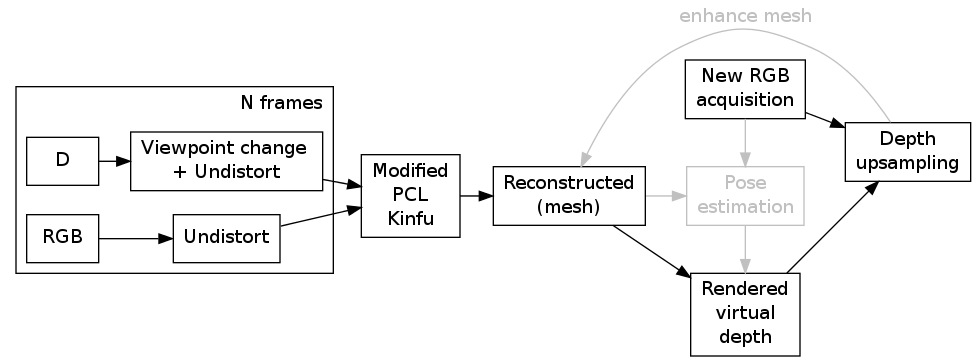
\includegraphics[width=\linewidth]{/home/bontius/workspace/cpp_projects/KinfuSuperRes/thesis/img/sys_overview.png}
    \caption{System overview}
    \label{fig:sys_overview}
\end{figure}

\par In \figref{fig:sys_overview} the overview of the designed solution is outlined. The main steps of the targeted system are as follows: (1) RGB-D acquisition and pre-processing, (2) 3D reconstruction, (3) new input acquisition and processing, (4) detail up-sampling and (5) mesh enhancement. Step (3) involves pose estimation of the new input. Ideally, this step enables high resolution RGB images to convey more information about details of the reconstruction. The pose estimation of a captured, high-resolution RGB image can be solved using methods in the area of multi-view stereo, for example bundle adjustment. This step was simulated in our project by the medium-resolution RGB images captured by the Kinect camera, where the pose estimation was performed by the Kinect Fusion algorithm. We thereby show, that there is information in the original input feed that can be used to improve on the output of the 3D reconstruction system. Substantial work was performed to enable mesh enhancement in step (5). However, some problems originating from the fact, that a re-sampling occurs when a 2D projection is created from the estimated pose could not be overcome in the frames of this project. Knowledge from the domain of geometry processing is to be involved to successfully merge the details rediscovered by our solution into the 3D reconstruction.

\par The system outlined above enables iterative refinement of the reconstructed model by acquisition of new input containing new information about the desired details.

\section{Assumptions}
\label{sec:assumptions}

\par When designing a system solving a specific problem, it is important to firmly decide what assumptions are made about the input, what problems are targeted to be solved and what problems are out of the scope of the planned method. We target to design a system, that reconstructs fine surface details of static scenes with mostly Lambertian surfaces allowing offline post-processing. \\

\par The fine surface details of a static scene are to be reconstructed. The problems arising when dealing with dynamic scenes are out of scope for this solution. Rigidity is a common assumption in the field of 3D reconstruction both for multi-view stereo and structured lighting methods. An essential building block of our concept is the possibility to later acquire new data about missing details and integrate it into the reconstruction. Since pose estimation of latter acquisitions is a substantial problem on its own, the assumption about static scenes seems reasonable to make. \\

\par Surfaces with close-to Lambertian reflectivity are considered. During experiments refractive and reflective surfaces appeared in the scene, but the main focus of the system development addresses problems emerging around fine details on mostly Lambertian surfaces. \\

\par The solution will perform post-processing offline. The planned key contribution of the work is to acquire surface details at a finer level than current state-of-the art solutions are capable of. As generally in all fields of computer science, a trade-off between quality and speed has to be made. Thus, the planned solutions operate using offline processing and refinement steps. Precedence in similar projects of using offline processing as capabilities of cloud computing has been observed in applications as Adobe Catch \citep{AdobeCatch} or Microsoft Photosynth \citep{Photosynth}. State-of-the art large-scale RGB-D reconstruction algorithms also may operate off-line, as \citep{Zhou:2013}. \\

\section{3D reconstruction}

The task of accurate real-time mapping of complex and
arbitrary indoor scenes in variable lighting conditions was claimed to have been solved by \citep{Newcombe11}. They list using only a
moving low-cost depth camera and commodity graphics hardware to their contributions as well. There have been made many improvements to the method since it's initial publication detailed in \secref{sec:kinfu}. We base the hypothesis of our work on the claim, that RGB-D reconstruction's attention to the complexity of the scenes can be developed further. Therefore, during the design of the system this algorithm was treated as baseline, its results were reproduced, carefully inspected and an attempt was made to improve upon them. During the extensive research performed to assess the capabilities of derivatives of this algorithm to reconstruct the targeted fine details we did rarely come across projects giving reason to attempt to reproduce their results instead, and treat them as baseline. However, in the future point-based fusion concepts introduced by \citep{keller13realtime} is worth taking into account to improve the starting point of our algorithm.

\begin{figure}[h!]\centering
	\begin{minipage}[b]{0.33\linewidth}
		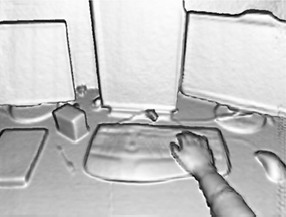
\includegraphics[width=\textwidth]{/home/bontius/workspace/cpp_projects/KinfuSuperRes/thesis/img/kinectfusion_example.png}
		\caption{Image from \citep{KinectFuSDKExample}}
		\label{fig:kinectsdk_example}
	\end{minipage}
	\begin{minipage}[b]{0.33\linewidth}
		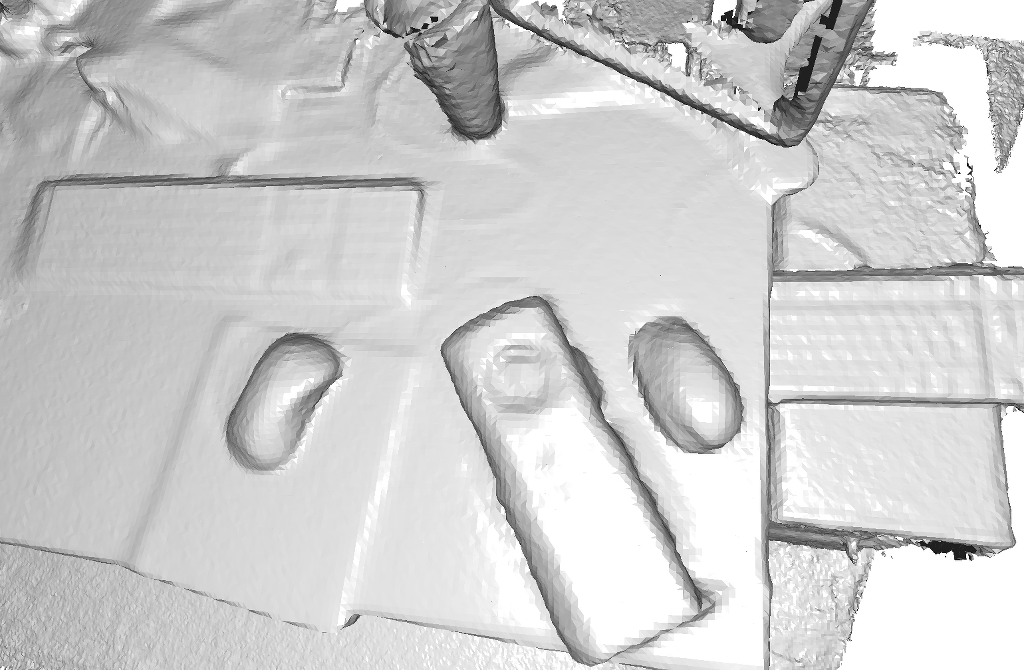
\includegraphics[width=\textwidth]{/home/bontius/workspace/cpp_projects/KinfuSuperRes/thesis/img/kinfu_baseline00.png}
		\caption{Mesh reconstruction of scene recorded by us. Reconstruction using PCL's Kinfu with our modifications}
		\label{fig:kinfu_baseline}
	\end{minipage}
	\begin{minipage}[b]{0.33\linewidth}
		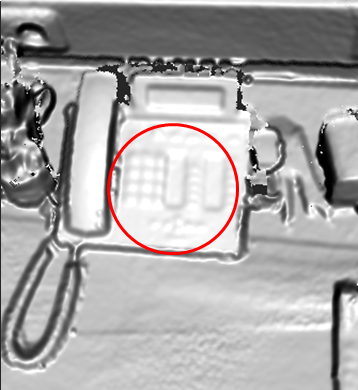
\includegraphics[width=\textwidth]{/home/bontius/workspace/cpp_projects/KinfuSuperRes/thesis/img/lefloch_largescale_cropped.png}
		\caption{\citep{keller13realtime}}
		\label{fig:lefloch}
	\end{minipage}
\end{figure}



\subsection{System input}
\par The system design applied in RGB-D SLAM 3D reconstruction methods aligns well to our initial concept of deign of solution. This is true both in terms of processing pipeline and hardware and software tools applied. The scene acquisition happens using sensors providing both chromatic and distance information. It is a common assumption to use a low-cost, usually hand-held device with integrated sensors as the Microsoft Kinect or ASUS Xtion Pro. A calibrated system of a time-of-flight camera and an RGB camera is another usual system setup. We used a calibrated Microsoft Kinect device. \\

\par An RGB-D SLAM 3D reconstruction system operates with at least two input streams. A data stream containing chromatic information about the observed scene, usually encoded in 8-bits per channel, and another information source conveying information about the spatial relations of the scene encoded in some form of distance information.
\par The Microsoft Kinect is capable of conveying three channels of chromatic data encoded in a 24-bit data-stream. The most important available resolution settings with the used OpenNI Middleware are 640 x 480 pixels at \mytilde 30 frames per second and 1280 x 1024 pixels at \mytilde 15 frames per second. The quality of the RGB image seems to suffer from the problems Bayer filtering type methods introduce, as it can be seen in \figref{fig:kinect_rgb_zoom}. This introduces slight corner detection problems at calibration time, and more significant problems when applying the up-sampling algorithm as discussed in the limitations section \secref{sec:limitations}. 
\par The depth stream is available in the resolution 640 x 480 at \mytilde 30 frames per second. The critical analysis of the quality of the depth map has been researched in many projects, amongst others by modelling the noise of the sensor \citep{NguyenIL12}, or applying temporal filtering \citep{RGBZcamera}. It is considered out of the scope of the current project to pre-process the depth stream before applying it in the system pipeline. \\

\par To establish working volume boundaries and area of focus, the operating range and optimal scanning distance of the used depth acquisition device has to be known. According to \citep{Kinect_ms} the Kinect depth sensor has a minimum range of 800 mm and a maximum of 4 m. The Kinect for Windows Hardware can work in Near Mode providing a range of 500 mm to 3 m. By sampling the depth maps acquired during our data collection process it can be stated, that these characteristics can be achieved using the OpenNI Middleware as well, depths around 500 mm have been observed. 
\par In future work, the \citep{Kinect_nyko_zoom} might provide possibility to zoom in further on the scene and acquire more accurate depth data about fine details, meanwhile the distortion effect of the additional lens has to be evaluated as well.

\subsection{Processing algorithm}
\par An open-source implementation of the classical Kinect Fusion algorithm was employed to retrieve a smooth 3D reconstruction from the data acquired. The \citep{PCL} has implementation both for the original small to mid-scale algorithm named "Kinfu" and an implementation capable of handling scenes with larger extent called "Kinfu Large Scale". Due to the targeted proof-of-concept nature of our project the computationally slightly less intensive Kinfu implementation was used as starting point. The sub-project was recompiled to a separate, modifiable library allowing slight customisations to the algorithm (project "MyKinfuTracker" in the source code attachment). Algorithmic changes or implementation of later publications detailed in \secref{sec:kinfu} incorporating improvements to the concept are considered out of scope for this project.\\

\par The outline of PCL's Kinfu algorithm is as follows: All depth data streamed from a Kinect sensor is merged into a global implicit surface model stored in a fixed resolution voxel grid in the GPU's memory. In each voxel grid cell the distance to the closest surface is stored as a truncated signed distance function (TSDF). Subject to convention the two signs represent the inside respectively outside of the assumed non-degenerate mesh. 
\par Upon arrival of new depth data a 3D point vertex and normal map is generated using camera the intrinsics. Correspondence to the stored mesh represented by the stored TSDF is calculated using ray-casting and the point cloud represented by the vertex map is used to estimate the new camera pose with respect to the current model. This is performed using a coarse-to-fine iterative closest point algorithm. 
\par The point cloud is then regenerated using the new camera pose and the appropriate cells of the voxel grid are updated. A new vertex and normal map is generated to prepare for the next arriving frame. The update method has large impact on our project goals. In \secref{sec:3d_sys_output} the role is discussed further with other parameters of the algorithm. \\

\par By recompiling PCL's Kinfu solution to a stand-alone library we prepared the implementation for future modifications. This allowed us to experiment with the different parameters detailed in the next section. These were hard coded into the solution in order to enable CUDA code to perform optimally. The most important modification besides change of parameters was to turn off the initial bilateral filtering of the input depth to enable higher attention to detail. The effectivity of this modification was suppressed by the averaging nature of the TSDF update method. Since the rest of the implementation assumed filtered depth maps with no missing information, a bilateral filtering step was reintroduced, that fills only pixels with missing data. A more accurate solution would require missing data to be disregarded at later stages of the pipeline.

\subsection{Configuration and system output}
\label{sec:3d_sys_output}

The results of the reconstruction stored in the voxel grid as a TSDF volume can be exported to several output formats. A GPU implementation of the classical marching cubes algorithm \citep{Lorensen:1987} exports the mesh into a point cloud. A triangle mesh can also be exported using the same method and connecting neighbouring grid cells to faces. The storage format is greedy storing all three vertices for every face. This introduced algorithmic challenges when performing subdivision on the mesh at later stages of the pipeline. The results can also be visualized using ray-tracing and Phong shading. We used the triangle mesh as output of this system in the pipeline.

\par Configuration parameters can be used to tweak the system to yield more optimal results, a reconstruction with higher attention to detail. The most important parameters of the Kinect Fusion algorithm are voxel grid resolution, working volume size, truncation distance, maximum movement threshold and weight of new information.

\par The resolution of the voxel grid and working volume size has the highest impact on the accuracy of fine details in the reconstruction. The parameters used during reconstruction resulted in a spatial resolution of $3 m / 512$ or $3 m / 640$ meaning an average accuracy of 5.85 mm respectively 4.68 mm. This implied a $3m^3$ working volume represented by $512^3$ respectively $640^3$ voxels. Higher values were bounded by hardware constraints (GPU memory size). The quality of the final output of our system was compared relatively to the output of the 3D reconstruction in the \secref{sec:discussion_results}.

\par The truncation distance has an impact on the accuracy of cavities and narrow details. The importance of this parameter is relevant when performing the raycasting steps of the algorithm. Since our solution does not need real-time performance this value could be increased to result in results with higher accuracy. Thus the output quality is not limited by this parameter, but by the spatial resolution of the voxel grid.

\par The maximum movement threshold is relevant to the pose estimation step of the algorithm. This parameter ensures, that the pose estimation algorithm did find a good match between the model and the new frame. By increasing the tolerance for movement between frames, we would allow less accurate pose estimations and faster camera movement. By decreasing the value more information would get discarded.

\par As stated earlier, the TSDF update method is an important parameter in terms of the reconstruction quality. In the given implementation, the information conveyed by new measurements are averaged giving each measurement equal weight. On the \citep{KinectFuSDKExample} page they say, that the weight parameter {\it "...controls the temporal averaging of data into the reconstruction volume – increasing makes the system a higher detailed reconstruction, but one which takes longer to average and does not adapt to change. Decreasing it makes the volume respond faster to change in the depth (e.g. objects moving), but is noisier overall."}. The equal weighting of all measurements has a large impact on the output introducing a strong smoothing effect discarding fine surface details and giving place to the hypothesis of our project.

\section{Depth super-resolution}

\par The base hypothesis of our project states, that there is information recorded by the sensors that is discarded early in the pipeline. We claim, that by identifying and reintegrating this information at later stages, it is possible to improve the reconstruction of fine surface details in comparison to existing 3D reconstruction methods. 

\par In \secref{sec:super_resolution} many image-, depth- and joint super-resolution methods were overviewed. The claimed power of the method published by \citep{cvpr-07-qingxiong-yang} served as basis for the main hypothesis of the project. In their works they demonstrate successful ten-fold up-sampling of noisy, low resolution time-of-flight depth images with the help of registered RGB images. Later works often refer to \citep{cvpr-07-qingxiong-yang} as super-resolution by joint bilateral filtering. However, the original method applies joint bilateral filtering in an iterative fashion on a cost-volume originally necessary for the stereo-matching problem targeted. The main hypothesis of cross-bilateral filtering says that neighbouring pixels that are spatially closer and similar in [colour] appearance are more reliable and thus to be given more weight when estimating a new value for the center pixel of the filtering kernel.
\par The two main contributions of their project emphasized in our solution is this neglected iterative nature of their method and the implementation of sub-pixel accuracy to the depth search range and its resolution. An overview of their algorithm can be seen in \figref{fig:yang_overview}. The full algorithm was reimplemented during the course of the project. Given its computational intensity, a full GPU implementation was developed further described in \secref{sec:implementation_details}

\begin{figure}[h!]\centering
    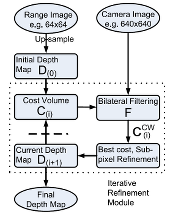
\includegraphics[width=0.4\linewidth]{/home/bontius/workspace/cpp_projects/KinfuSuperRes/thesis/img/yang_overview.png}
    \caption{System overview of \citep{cvpr-07-qingxiong-yang}}
    \label{fig:yang_overview}
\end{figure}

\subsection{System input}

\par The system takes two registered images as input. One of the images is the depth information targeted for up-sampling. This image is supposed not to contain details to the desired scale. The second input is a colour image conveying the extra information used for enhancement. By applying the method described, the depth image can be up-sampled to the same resolution as the colour image. The exact registration of the images has proven itself to be of high importance. The system is also sensitive to several parameters as input, described in the next subsections.

\subsection{Processing algorithm}
\par The depth image is up-sampled to the resolution of the RGB image, and
serves as the initial hypothesis of the depth information. In our implementation a nearest neighbour strategy is applied to reduce the number of possible sources of artifacts. 
\par Afterwards, an iterative refinement process is started. First a cost volume is built based on the current depth estimate. For every pixel, every depth hypothesis within a relatively narrow search range is compared to the current hypothesis. The cost of the investigated depth value depends on the distance from the current hypothesis subject to a cost function. The algorithm uses a truncated quadratic cost function to enable large depth discontinuities, meanwhile ensuring a smooth gradient search.
\par Then joint bilateral filtering is applied to the cost volume to handle artifacts in the proximity of large gradients. The necessity of this step is supported by an undesired fattening effect around edges. By applying bilateral filtering the compatibility of the new depth value to its neighbourhood is investigated. This compatibility is modulated by the spatial distance between the neighbouring pixel subject to a Gaussian fall-off, and the distance in appearance also subject to a Gaussian fall-off with different variance.
\par After filtering the cheapest new depth value is selected by a winner-take-all strategy. Then the cost of the two neighbouring hypotheses are used to perform a sub-pixel estimation procedure to enhance the resolution determined by the search step during the construction of the cost volumes.

\par The stop condition is not described in the original paper, but the published datasets allow us to conclude that around 130 iterations were performed on depth data in the 0..255 range. Since our depth images usually lie in a larger range of 0..3000, a minimum-average-difference stop condition was tested in the implementations. Finally we decided to fix the allowed change of a depth value based on the assumption, that we can assume a maximum change in mm-s given the targeted scene.

\subsection{Configuration and system output}

\par The algorithm is moderately sensitive to several parameters that need to be adapted to the domains of the current problem. The highest sensitivity is introduced through the joint bilateral filtering. 

\par The variance of the two Gaussian fall-offs are to be set. The current solution operates with fixed variances, and the adaptivity to the characteristics of the input data is accomplished through the fact, that the appearance information is taken into account during the filtering. High spatial variance can be interpreted as a larger smoothing filter granting influence to more distant neighbours in the filter kernel. Low spatial variance dampens the smoothing effect to the cost of the effectivity of the filtering. A future improvement to our algorithm is to automatically calculate the maximum necessary filter kernel size from this variance (an often seen heuristic is to set it to two times the standard deviation), currently it's set separately.
\par The variance of the Gaussian responsible for assigning weights to neighbours based on appearance information is also an input parameter. A high variance can be interpreted as being more allowing regarding the appearance of the neighbours. This is favourable if the quality of the colour input is low. Low variance means being very restrictive and assuming good input quality where object similarity is well captured by the colour information. The original algorithm applies an equally weighted gray scale conversion. In future work the effect of not discarding hue information should be investigated. Given the low quality of the high resolution RGB images returned by the Kinect's camera, the gray scale conversion was a necessary decision.

\par Bilateral filtering methods usually allow several iterations to be performed to handle data with higher noise levels. The effect of this can be translated to a larger kernel size and thus only one iteration of filtering was performed on each slice of the cost volume. This decision is also supported by the fact, that the whole algorithm relies on an iterative concept.

\par The iterative up-sampling algorithm relies on parameters determining the truncation of the cost function, the search range and its resolution and the fixed maximum iteration count implementing the stop condition. A lower truncation level of the quadratic cost function is desired to preserve large depth discontinuities in the scenes. The search range is quite statically determined by the depth domain of the scene, and is recalculated at each iteration to speed up computations. The range is set to contain the current depth spectrum padded by the truncation value of the cost function. 

\par The search step parameter determines the maximum possible accuracy of the method without the sub-pixel refinement. It was set to 1 mm in during experiments. A value inherited from the fact, that the input depth data is provided encoded as 16 bit integers with mm precision. The calculations in the pipeline are performed on float data, and due to the sub-pixel accuracy calculations, have not too large impact. The interpretation of the search step is, that a quadratic function is fitted using three samples spaced by the search step. This gives a hard to interpret notion of accuracy.

\par In the original paper there is no mention of representation errors or limitation of the sup-pixel accuracy estimation due to close to zero divisions. In our implementation a salt-pepper like noise was observed close to very large edges. Therefore a change limitation was introduced to bound the output of the sub-pixel estimation step to the range $\pm 1 \cdot search\_step$.

\par The output of the algorithm is demonstrated in the validation chapter \chpref{chp:validation}. The validity of the reimplementation is also tested on the datasets attached to the original publication.
        
\section{Combined system pipeline}
\label{sec:combined}

\par The designed system accomplishes the targeted high-resolution 3D reconstruction by combining the above outlined two systems, smooth 3D reconstruction and depth up-sampling. The overview of the constructed system is shown in \figref{fig:sys_overview}. A very important concept in the designed solution is the possibility of including new data to enhance parts of the reconstruction previously not sufficiently observed. This allows for a freedom to combine sensors and their characteristics. This theoretical design feature was tested by using the existing acquired data to check, whether there is unused information not picked up by the initial reconstruction. The pose estimation of the Kinect Fusion algorithm is used to render a new depth image of the reconstructed model from a simulated virtual viewpoint. Since the pose is known, the aligned RGB data can be used to up-sample the depth from the virtual viewpoint.

\subsection{Pre-processing the input}

\par To ensure high quality alignment required by the later parts of the pipeline a extensive work was performed to gather information about the extrinsic and intrinsic parameters of the recording device. 10-component intrinsic parameters for both lenses were calculated alongside with the estimation of the extrinsics connecting the two cameras. Further details are discussed in \secref{sec:calibration}.

\par The estimated camera parameters are used to remove lens distortion from both input streams and to reduce the two coordinate systems to one by mapping the viewpoint of the depth camera to the coordinate space of the RGB camera. By doing this before the streams are provided to the smooth reconstruction algorithm a compromise is made. The mapping calculations introduce estimation errors, loss of depth data by occlusion in the new viewpoint and representation problems due to the non-rectangular output of the distortion removal algorithms. The gain is to be able to use the aligned input feeds for further, quality enhancing pre-processing algorithms, for example joint-bilateral filtering. The strong smoothing effect of the 3D reconstruction algorithm applied takes away the edge of this gain, in future work the viewpoint mapping is to be moved to after the smooth reconstruction step.

\subsection{Rendering a virtual viewpoint}

\par After the smooth 3D reconstruction, any virtual viewpoint of the system has to be possible to render. Therefore, the results of the reconstruction have to be stored. Furthermore the projection parameters of the virtual viewpoint have to match the characteristics of the capturing device that the newly acquired data was recorded with. The actual rendering of the model representation has to be performed, and information about the sampled parts of the mesh has to be collected.

\par The calculation of the actual position of the virtual viewpoint is detailed in the future work section \secref{sec:future_work}. Bundle adjustment implemented in \citep{SnavelySS06} or \citep{vsfm} can be used to align the new RGB data with the available snapshots from the Kinect stream. The new sparse and stored dense reconstruction model can than be aligned, so that the estimated new camera pose can be transformed between the two coordinate systems.

\par To  store the results of the smooth reconstruction in a loss-less fashion the data structure of the Kinfu implementation is to know. The 3D voxel grid is mapped to a 2D storage array in the GPU memory. In order to be able to perform a large variety of sampling operations on the results the original grid was saved to disk using existing tools. The read-back to GPU memory had to be implemented. The exact storage of the TSDF volume enables ray-casting to be performed to render the virtual viewpoint. Using the marching cubes algorithm the theoretical accuracy of this representation is approximated. However by storing triangle meshes in PLY format a wider range of existing rendering tools became available and calculation times were heavily reduced. This practical separation of the pipeline can be reversed in future work. The loss of accuracy was attempted to be counter-weighted by the employment of different mesh subdivision algorithms. The sub-optimal data structure of the triangle mesh is not compatible with the available existing subdivision implementations. Since this algorithmic step will prove unnecessary in future work, further attention was not given to the problem arising through an earlier approximation step.

\par To render the virtual viewpoint of the reconstructed model three different approaches were developed. PCL's octree implementation allowed the quick development of a ray-casting algorithm. The execution was performed on the CPU very similarly to the Kinfu GPU algorithm, thus the projection parameters involving the used camera intrinsics were closely controlled. The information about visible vertices and faces is easily retrievable using this method as well. This information is needed by the mesh enhancement step, where the modified primitives have to be merged with the unmodified primitives of the mesh. Unfortunately our meshes consisted of 1.5 - 2.5 million vertices which made the CPU implementation too slow despite the effective octree point cloud representation. Problems arised in form of the hand-tuning of the maximum octree grid resolution and the need to account for larger faces occluding rays but not represented by the octree structure.

\par GPU based renderers of triangle meshes are widely known. PCL relies on the library called \citep{vtk}. Unfortunately in its newest version the possibility to specify all elements of the projection matrix independently is not enabled. Therefore, after many attempts to use the offered interface to accomplish the incorporation of the exact intrinsics into the rendering system a third method had to be discovered. Visibility information is also not retrievable using this method.
\par A GLSL based rendering environment was implemented to ensure full control over the projection parameters, quick rendering of the large number of input triangles, and full information about appearing vertex- and face ids. A FramebufferObject is set as render target, the depth buffer texture is read and rescaled to retrieve the depth map, and unclamped unsigned textures are attached as fragment shader outputs to retrieve information about sampled vertices and faces.

\subsection{Model enhancement}
\par Several strategies were developed to accomplish the substitution of the projected vertices and faces by the up-sampled depth data. It is established, that the re-sampling nature of the problem requires solutions to be imported from the geometry processing domain. Operations like this were considered out of scope for the current project.

\par As results the up-sampled 2D depth maps containing some desired and other unwanted high-frequency details are rendered as 3D point clouds and triangle meshes using the naive parametrisation provided by the pixel grid of the 2D image. Further details in \secref{sec:results}.

\section{Calibration}
\label{sec:calibration}

\par In the previous sections it was established that correct alignment of the input sources shown in \figref{fig:input} has to be executed to enable the up-sampling algorithm to perform. In \figref{fig:calib_built_in} the built-in calibration is shown to be not accurate enough. This calibration is provided by the OpenNI middleware and is stated to be read from the hardware chip of the recording device. By paying attention to narrow non-gray areas (IR occlusions) in the image one can observe the misalignment of the contours of the images.

% Input rgb and depth
\begin{figure}[h!]\centering
    \begin{minipage}[b]{0.49\linewidth}
        \includegraphics[width=\textwidth]{/home/bontius/workspace/cpp_projects/KinfuSuperRes/SuperRes-NI-1-5/build/out/imgs_20130725_1809/img8_00000001.png}
    \end{minipage}
    \begin{minipage}[b]{0.49\linewidth}
        \includegraphics[width=\textwidth]{/media/Storage/Dropbox/UCL/project/results/presentation_300713/dep8_00000001.png}
    \end{minipage}
    \caption{Input RGB and depth from Microsoft Kinect camera}
    \label{fig:input}
\end{figure}

% Simple alignment
\begin{figure}[h!]\centering
	\begin{minipage}[b]{0.49\linewidth}
		\includegraphics[width=\textwidth]{/media/Storage/Dropbox/UCL/project/results/presentation_300713/dep16AndRgb_00000001.png}
	\end{minipage}
	\begin{minipage}[b]{0.49\linewidth}
		\includegraphics[width=\textwidth]{/media/Storage/Dropbox/UCL/project/results/presentation_300713/dep16AndRgb_00000000.png}
	\end{minipage}
	\caption{No alignment superposition and "Built-in alignment" from OpenNI Middleware}
	\label{fig:calib_built_in}
\end{figure}

\par The calibration procedure was performed between "raw" images captured by the IR camera and the colour images captured by the RGB camera. Approximately 70 images of both sources were annotated for user-supported corner detection. The calibration images were taken with the structured light projector covered, since that introduces intolerable noise to the corner detection performed on the IR images. Therefore a space with plenty ambient IR lighting (sun light) had to be used for the calibration. The calibration images were taken at several distances to ensure coverage of the whole working volume. Different perpendicular and skew angles were recorded covering the whole, and several sub-parts of the view area. A real-time visual feedback loop was developed to ensure that the full checker-board pattern is visible on both images. Pixel re-projection errors below 0.5 pixels were targeted to reach "sub-pixel accuracy". An A3 format checker-board was the smallest size yielding good enough results (evaluated qualitatively). For future work even larger formats are suggested. The printing method should stretch the paper as little as possible, and the calibration pattern should be attached to a perfectly flat surface with extra caution to  perfect alignment to the surface.

\par Extra attention was paid to the information available about the transformation algorithm that the Primesense sensor uses to convert the IR data to the provided depth images. According to several blog sources the width of the width of the output depth image is a result of 9x9 kernel up-sampling of the raw IR image. Therefore the calibration results were tested using this \mytilde 4.5 pixel offset. The accuracy of the reached calibration did not allow us to determine whether this makes sense. Some errors were corrected, some others were introduced as it can be seen in \ref{fig:calib_ir_depth}


\begin{figure}[h!]\centering
    \begin{minipage}[b]{0.49\linewidth} 
        \includegraphics[width=\textwidth]{/media/Storage/Dropbox/UCL/project/results/presentation_300713/irAndDep8_00000001.png}
        \caption{Default IR and depth overlay. A suspected offset of 4 pixels was examined.}
        \label{fig:ir}
    \end{minipage}
    \begin{minipage}[b]{0.49\linewidth}
        \includegraphics[width=\textwidth]{/media/Storage/Dropbox/UCL/project/results/presentation_300713/offsIrAndDep8_00000001.png}
        \caption{IR offset by radius of supposed convolution kernel. Some edges improve, some worsen.}
            \label{fig:calib_ir_depth}
    \end{minipage}
\end{figure}

\par Using the \citep{calibration_bouguet} the intrinsic parameters were estimated of both lenses. The calibration includes parameters skew ($\gamma$), radial distortion up to the third-order ($k_1$,$k_2$,$k_3$) and tangential distortion up to second-order ($t_1$,$t_2$). The extrinsic relationship between the two cameras was established as well. The \mytilde 30 mm translation between the two cameras seemed to be plausible results. Skew was hardly detected in any of the cameras, but the third-order radial distortion was \mytilde 0.5 for both cameras. The final re-projection error for the RGB camera was in the 0.1 pixel magnitude, the IR intrinsic calibration resulted in re-projection errors of 0.3 pixels. Since the re-projection is subject to the errors of the corner detection as well, these results were considered successful. The final alignment after viewpoint mapping and lens distortion removal can be seen in \figref{fig:final_calib}.

\begin{figure}[h!]\centering
        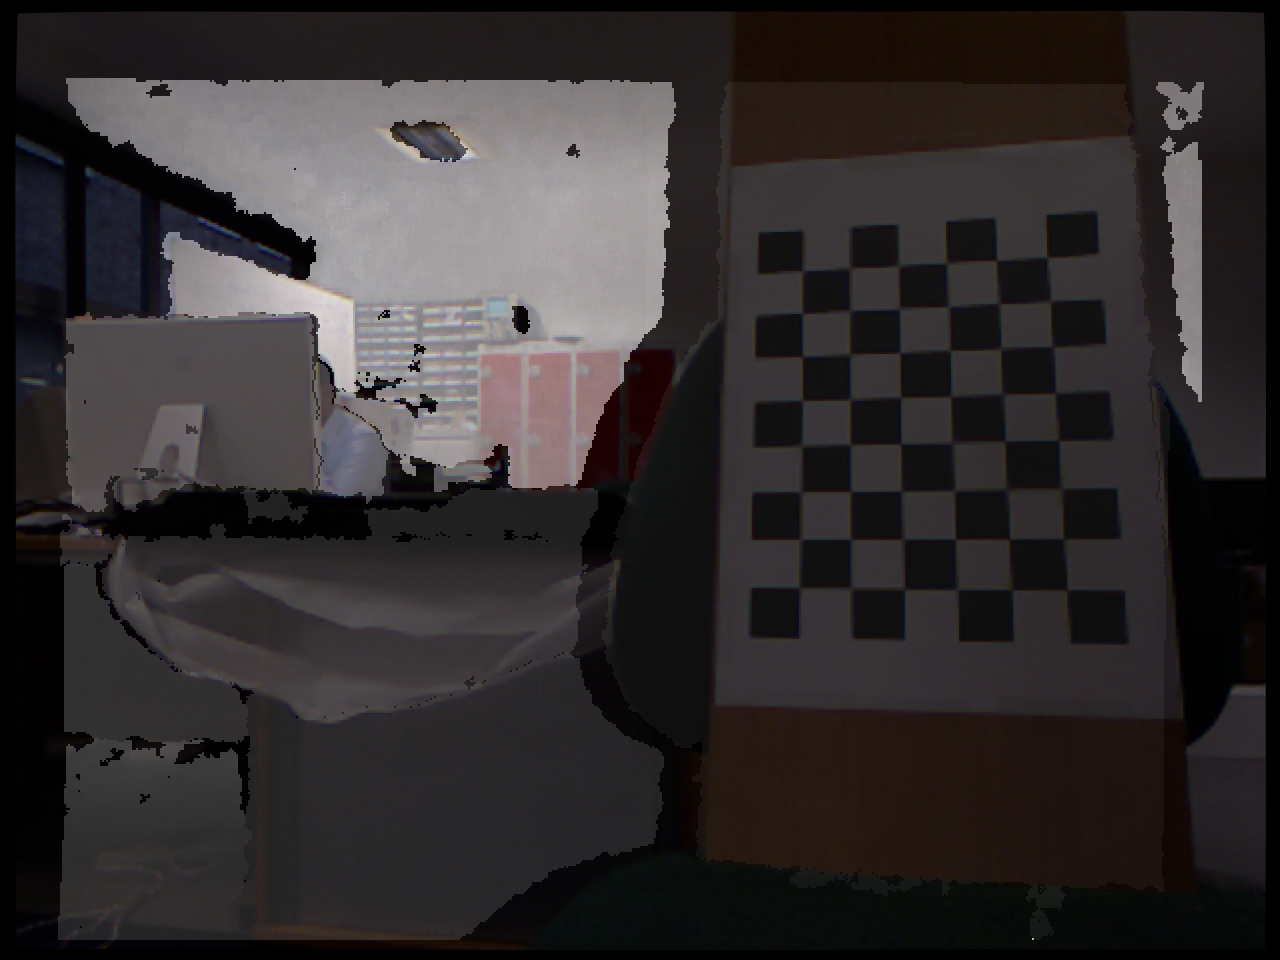
\includegraphics[width=\linewidth]{/home/bontius/workspace/cpp_projects/KinfuSuperRes/thesis/results/blendedUndistortedUC3x2.png}
        \caption{Mapping from 640x480 depth to 1280x1024 RGB after calibration and distortion removal}
        \label{fig:final_calib}
\end{figure}

\par The mapping algorithm implemented in the toolbox runs in the MATLAB framework. The mapping of a 640 x 480 depth image to the 1280 x 960 RGB image took around 1 minute to calculate for each frame. Therefore CUDA code from \citep{kinect_lua} was rewritten to perform the mapping and undistortion with speeds of the 1 ms magnitude for a frame.

\section{Implementation details}
\label{sec:implementation_details}

\par The solution implemented in C++, CUDA and GLSL was split into several libraries and projects connected, with cross-compilable CMake build configurations. Especially important for quick prototype development and testing was the Thrust implementation of the iterative, cost-volume based joint bilateral filter, that had to be replaced by an even more effective CUDA implementation. The viewpoint mapping algorithm was also implemented in CUDA to enable real-time testing and feedback. The Ubuntu operating system was used to benefit from the power of the open-source community.

\par The Microsoft Kinect SDK and Kinect Fusion SDK, and the two unix based middleware frameworks libFreenect and \citep{openni} were tested, and the OpenNI 1.5 legacy middleware was selected to enable the quickest development with the highest level of service. Source code from NVIDIA CUDA Samples, PCL example projects, \citep{DCBGridStereo} and \citep{kinect_lua} were used.

\par Additional common third-party libraries widely used in the project are: \citep{opencv} and \citep{libeigen}. Renderings shown in the figures in the document were made using \citep{Meshlab}.

%%% CHAPTER 5 %%%
\chapter{Experiments}
\label{chp:validation}

We targeted to build a system, that proves the hypothesis, that there is information discarded early in the 3D reconstruction pipeline and that it can be reintroduced later. The developed system also enables additional, possibly more detailed input to be captured and added the reconstruction later. The outline of the algorithm to be validated is repeated in \figref{fig:sys_overview2}.

\begin{figure}[h!]\centering
    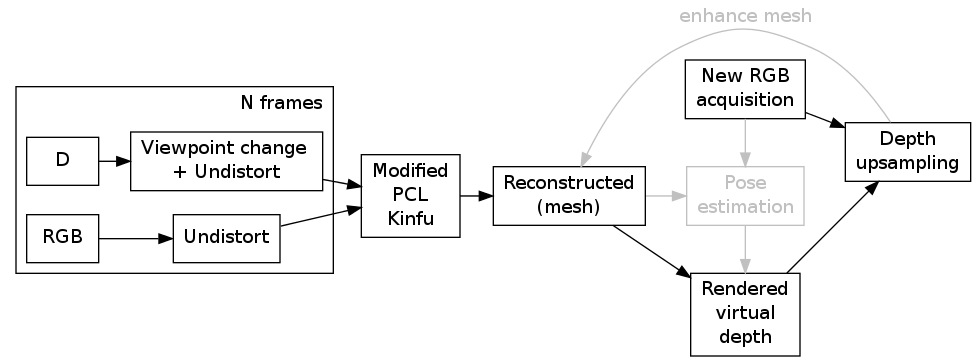
\includegraphics[width=\linewidth]{/home/bontius/workspace/cpp_projects/KinfuSuperRes/thesis/img/sys_overview.png}
    \caption{System overview}
    \label{fig:sys_overview2}
\end{figure}

The distortion removal and alignment of the input data was validated in \figref{fig:final_calib} and \figref{fig:limit_kinfu_pose}. The smooth reconstruction was tested extensively during mesh subdivision experiments. The successful rendering from a virtual point of view is demonstrated in \figref{fig:pose_138_in_out} on the left side. The reimplementation of the discussed depth super-resolution algorithm as one method of reintegrating discarded information is checked in \figref{fig:sofa}, \figref{fig:umbrella}, \figref{fig:chair}, and \figref{fig:pink}. The final output of the system is shown in \secref{sec:results}.

%%% SECTION results %%%
\section{System output}
\label{sec:results}

\par Several recordings have been made scanning a detail-rich desktop environment. The scenes contain diffuse surfaces, textured surfaces, transparent surfaces and reflective surfaces as well. As stated among assumptions, our primary focus was on close to Lambertian surfaces. 
\par The output of our system are up-sampled depth images with possible resolutions up to the input resolution of the RGB images. To ensure minimum loss of accuracy and portability, the output is saved as ASCII float matrix with extension the extension PFM. These images are then rendered in 3D using the calibrated camera intrinsics. The rendering outputs are provided in the format PLY. Both point clouds and naive triangle meshes are rendered. The naive triangle rendering supposes, that the depth image coordinate grid is a uniform parametrisation and connects neighbouring triplets to non-overlapping triangles. Some rendering artifacts due to large pixel discontinuities are considered side effects of the visualisation, and originate in non-perfect parameter settings of our method. Textured point clouds and triangle meshes are also rendered to show the origin of estimation errors. Some of the results of the system can be seen in \figref{fig:keyboard_192_final}, \figref{fig:keyboard2_192_final}, \figref{fig:pose_138_in_out}, and \figref{fig:pose14}. For some of the outputs' rendered meshes, please see attachment. The results are discussed in \chpref{chp:discussion}.

\begin{figure}[h!]\centering
    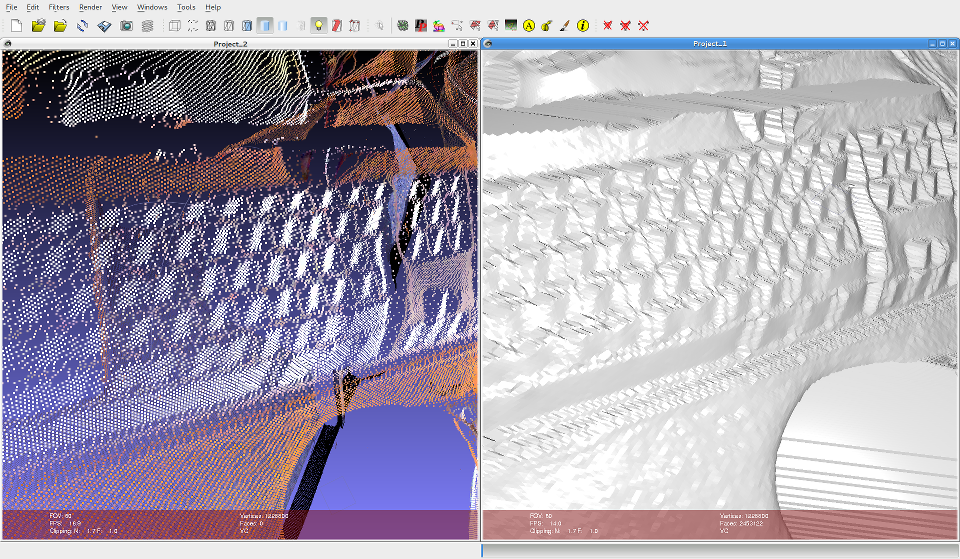
\includegraphics[width=\linewidth]{/home/bontius/workspace/cpp_projects/KinfuSuperRes/thesis/img/keyboard_192_final.png}
    \caption{Close up rendering of keyboard upsampled from skew view angle. Output textured point cloud and output rendered naive triangle mesh. Frame 192.}
    \label{fig:keyboard_192_final}
\end{figure}

\begin{figure}[h!]\centering
    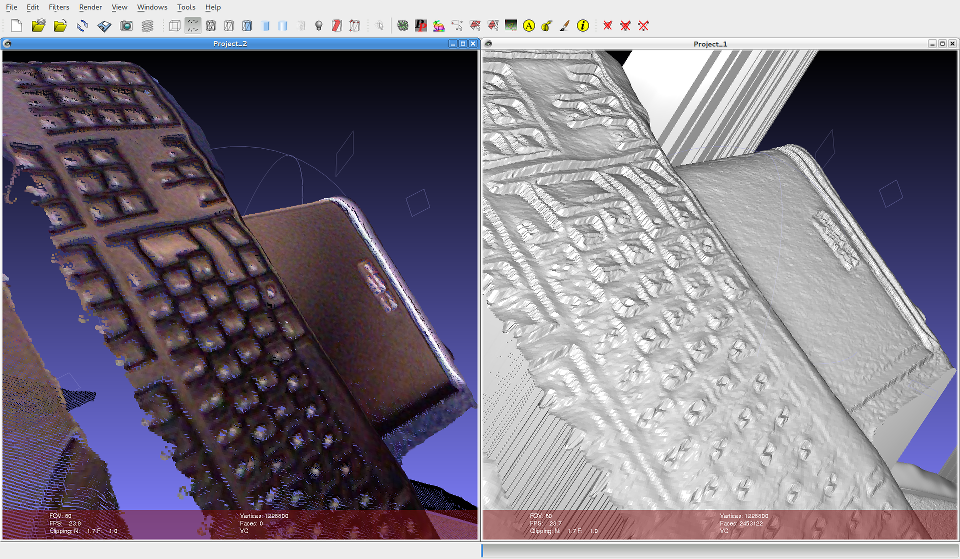
\includegraphics[width=\linewidth]{/home/bontius/workspace/cpp_projects/KinfuSuperRes/thesis/img/keyboard2_192_final.png}
    \caption{Close up rendering of different keyboard upsampled from closer to normal view angle. Output textured point cloud and output rendered naive triangle mesh. Frame 192.}
    \label{fig:keyboard2_192_final}
\end{figure}

\begin{figure}[h!]\centering
    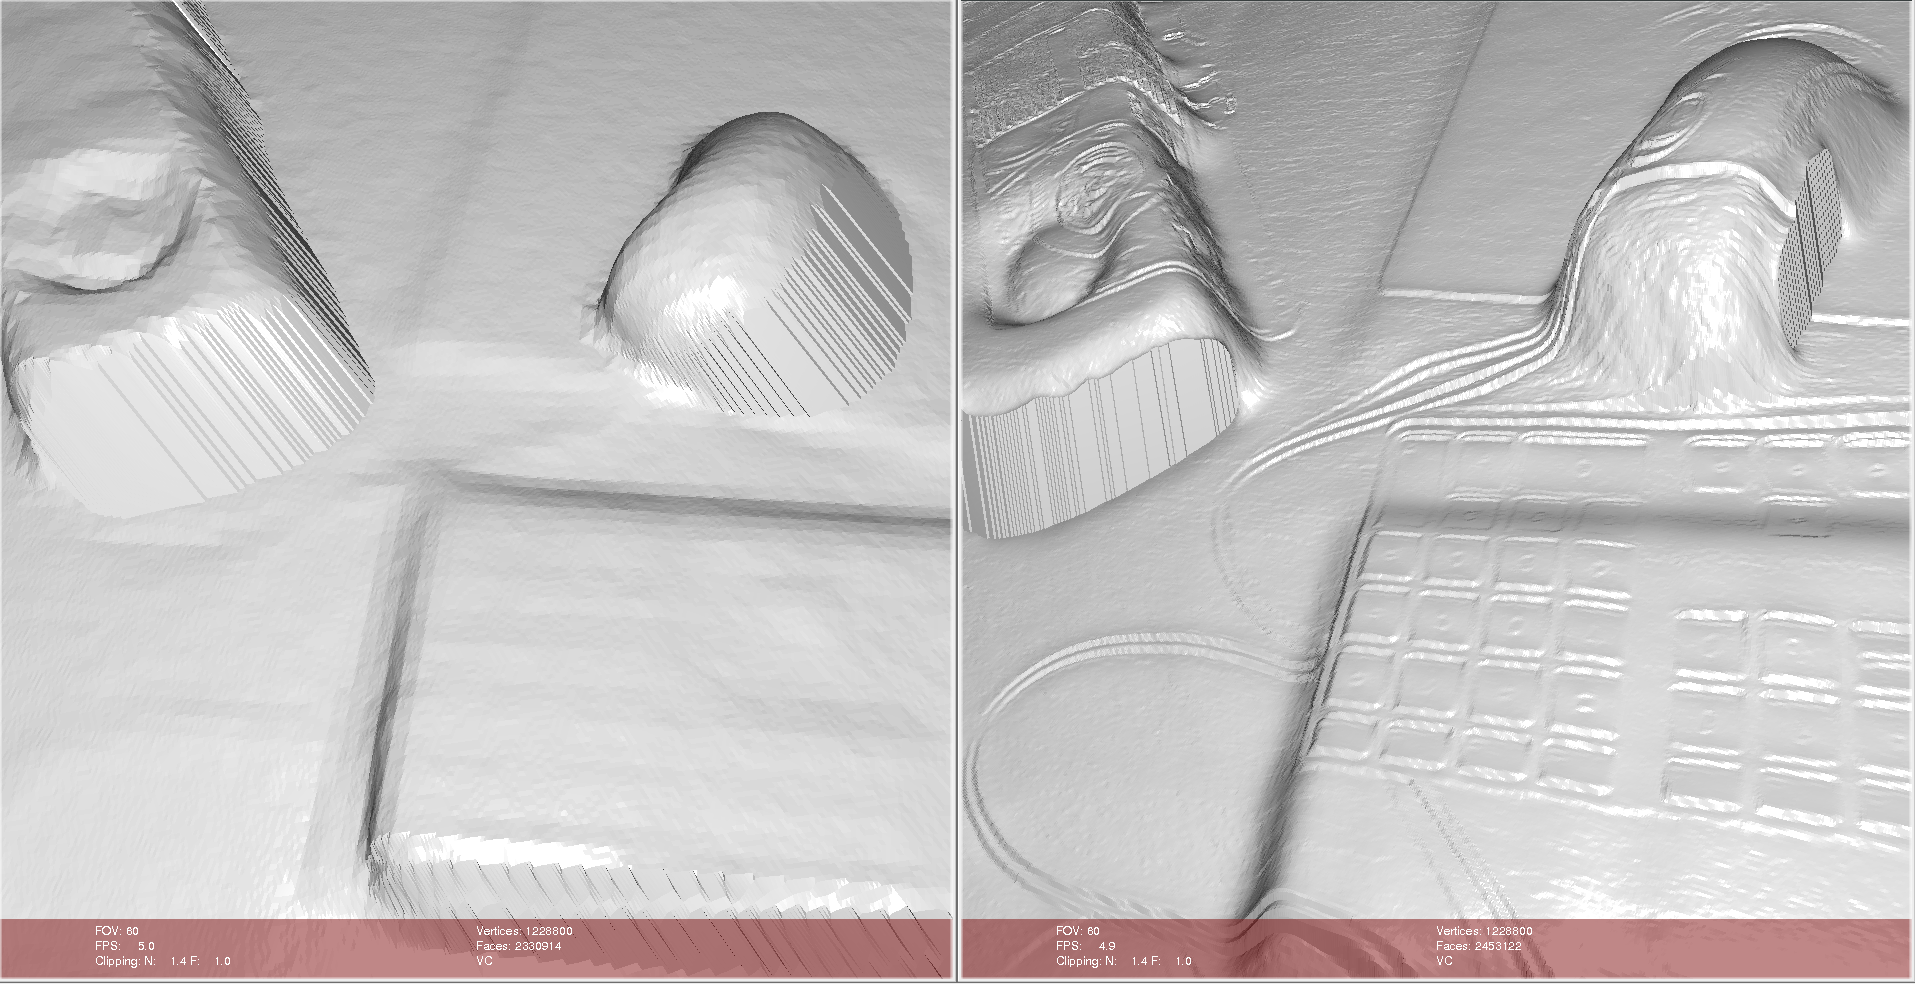
\includegraphics[width=\linewidth]{/home/bontius/workspace/cpp_projects/KinfuSuperRes/thesis/img/138_in_out.png}
    \caption{Close up rendering of keyboard and graphics card. Left: rendering from virtual point view; Right: output rendered naive triangle mesh. Frame 138.}
    \label{fig:pose_138_in_out}
\end{figure}

\begin{figure}[h!]\centering
    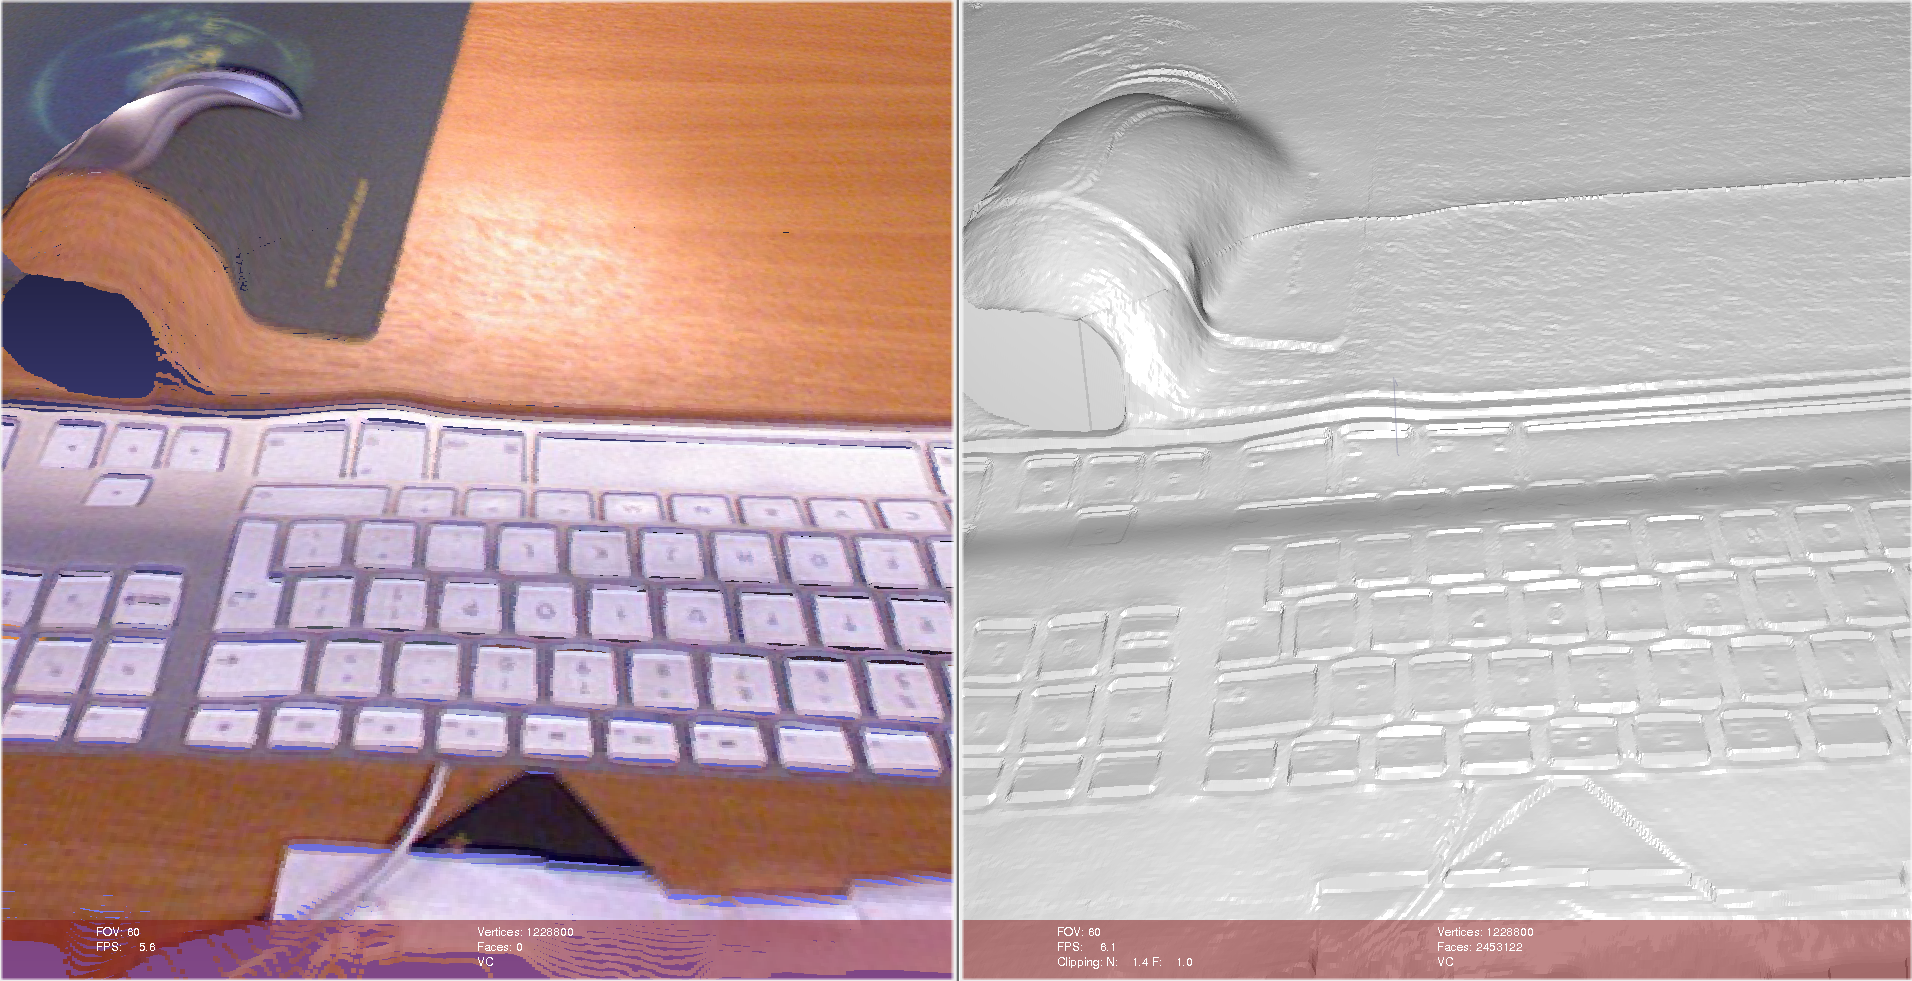
\includegraphics[width=\linewidth]{/home/bontius/workspace/cpp_projects/KinfuSuperRes/thesis/img/pose14.png}
    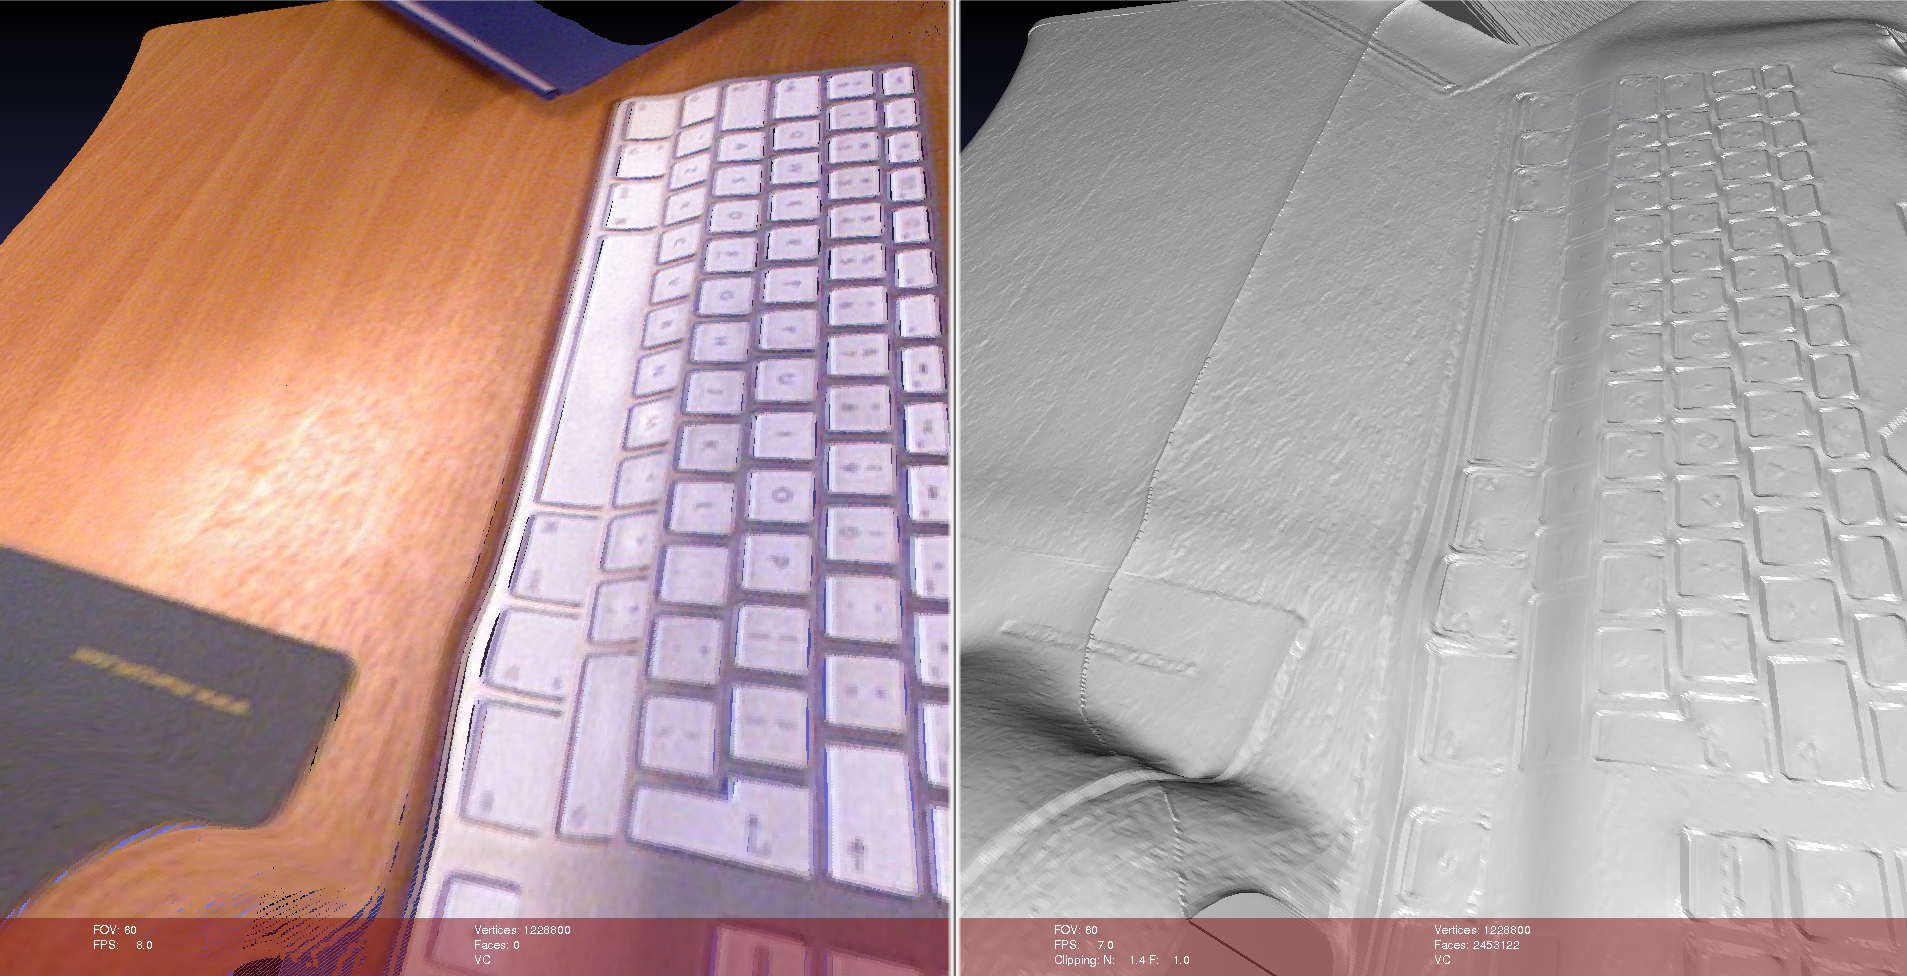
\includegraphics[width=\linewidth]{/home/bontius/workspace/cpp_projects/KinfuSuperRes/thesis/img/pose14_2.png}
    \caption{Effect of non-geometrical edges. Output textured point cloud and output rendered naive triangle mesh. Frame 14.}
    \label{fig:pose14}
\end{figure}

%%% SECTION %%%
\section{Iterative joint bilateral up-sampling with sub-pixel accuracy}
\label{sec:yang}

\par The second part of the pipeline consists of the re-implementation of the work published by \citep{cvpr-07-qingxiong-yang}. To explore the limits of the method and to verify the correctness of the implementation several experiments were executed. One of the methods biggest limitations are depth changes introduced by non-geometric edges in the RGB images. To test this, the an aligned RGB-D input of a checker-board pattern was served as input to the CUDA implementation of the algorithm. The result can be seen in \figref{fig:yang_checkerboard}. 
\par When designing the system an assumption was made that this depth up-sampling method reintroduces information to the scene from the RGB image. During initial tests, this assumption seemed to change characteristics. The current assumption is that the method is only capable of correcting depth values in the range of the observed depths. Not even the sub-pixel accuracy element ensures that new, unseen depths are introduced. Therefore a synthetic test was set up to understand the capabilities of the algorithm. The same checker-board RGB image responsible for \figref{fig:yang_checkerboard} was paired with a depth image of constant depth. As suspected, the result yielded an unchanged depth map, no new depth values were introduced outside the observed range of depth values.

\begin{figure}[h!]\centering 
        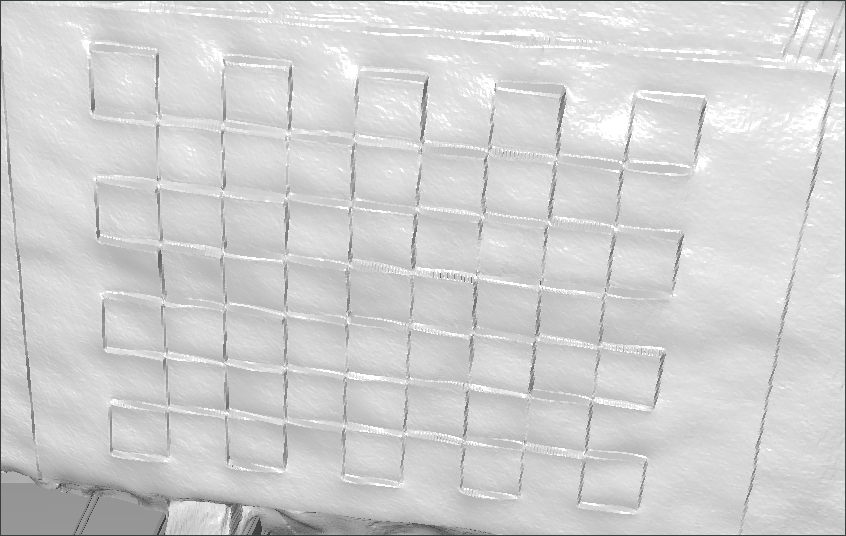
\includegraphics[width=\linewidth]{/home/bontius/workspace/cpp_projects/KinfuSuperRes/thesis/img/checkerboard.png}        
        \caption{Example run of implementation on checker-board scene, results without and with texture after 50 iterations.}
        \label{fig:yang_checkerboard}
\end{figure}

To make sure, that the above experiences are not due to a faulty implementation of the method, some the available inputs from the original dataset were processed, all with success. \figref{fig:sofa}, \figref{fig:umbrella}, \figref{fig:chair}, \figref{fig:pink}

\begin{figure}[h!]\centering
	\begin{minipage}[b]{0.49\linewidth}\centering
		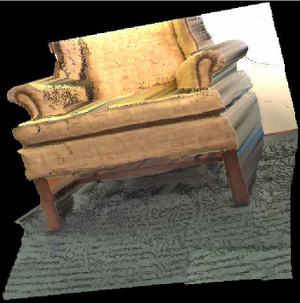
\includegraphics[height=5cm]{/home/bontius/workspace/cpp_projects/KinfuSuperRes/thesis/img/sofa_gt.png}
	\end{minipage}
	\begin{minipage}[b]{0.49\linewidth}\centering
		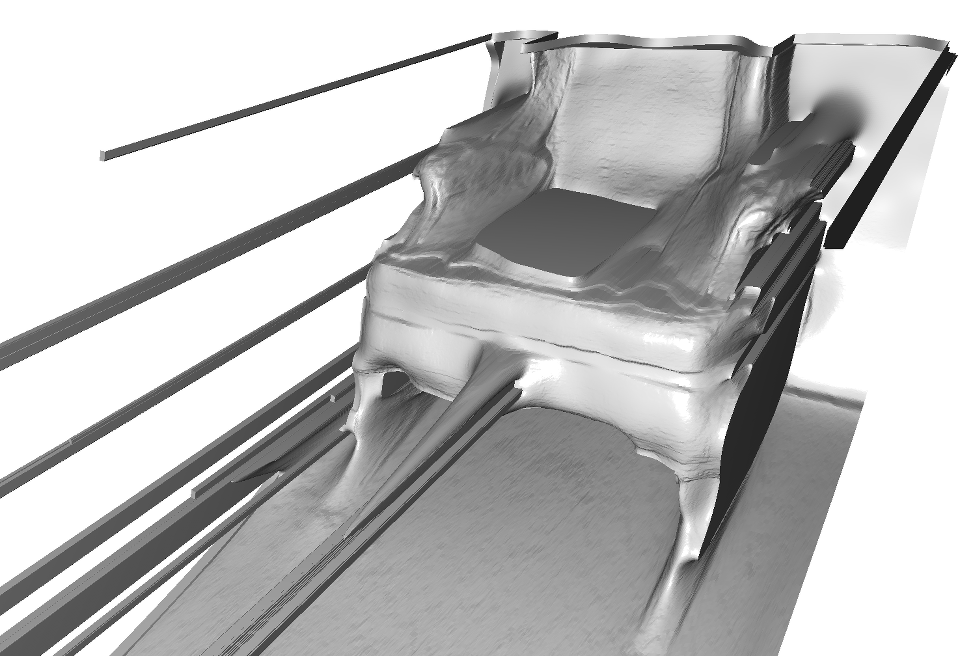
\includegraphics[height=5cm]{/home/bontius/workspace/cpp_projects/KinfuSuperRes/thesis/results/sofa00.png}
	\end{minipage}
	\caption{"Sofa" output by original paper (left) and by our implementation(right). Some artifacts due to untuned range variance.}
	\label{fig:sofa}
\end{figure}

\begin{figure}[h!]\centering
	\begin{minipage}[b]{0.49\linewidth}\centering
		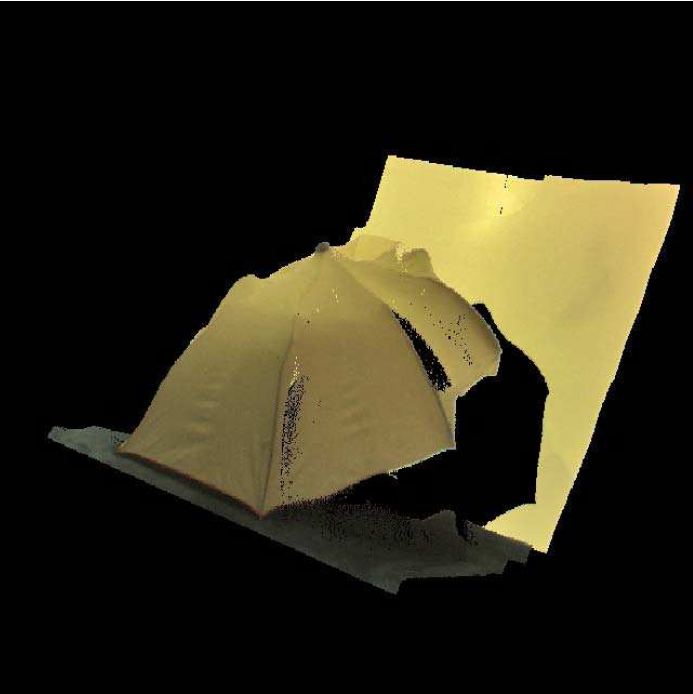
\includegraphics[height=5cm]{/home/bontius/workspace/cpp_projects/KinfuSuperRes/thesis/img/umbrella_gt.png}
	\end{minipage}
	\begin{minipage}[b]{0.49\linewidth}\centering
		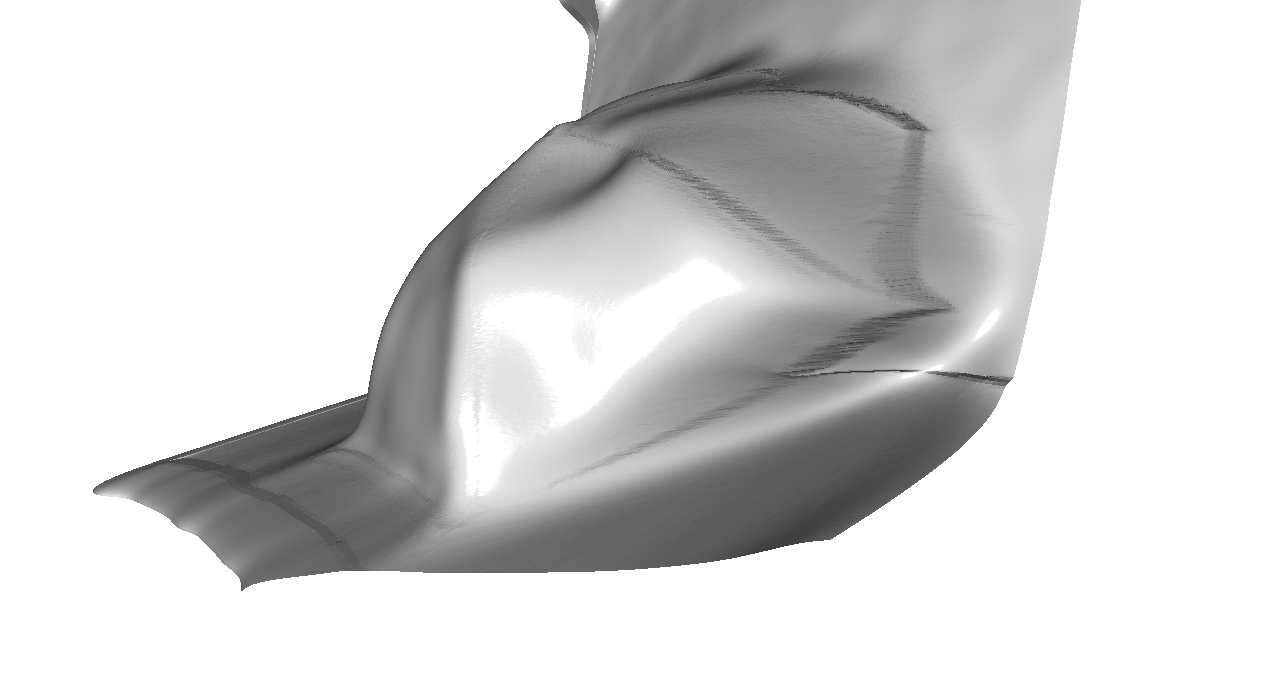
\includegraphics[height=5cm]{/home/bontius/workspace/cpp_projects/KinfuSuperRes/thesis/results/umbrella00.png}
	\end{minipage}
	\caption{"Umbrella" output by original paper (left) and by our implementation (right).}
	\label{fig:umbrella}
\end{figure}

\begin{figure}[h!]\centering
	\begin{minipage}[b]{0.49\linewidth}\centering
		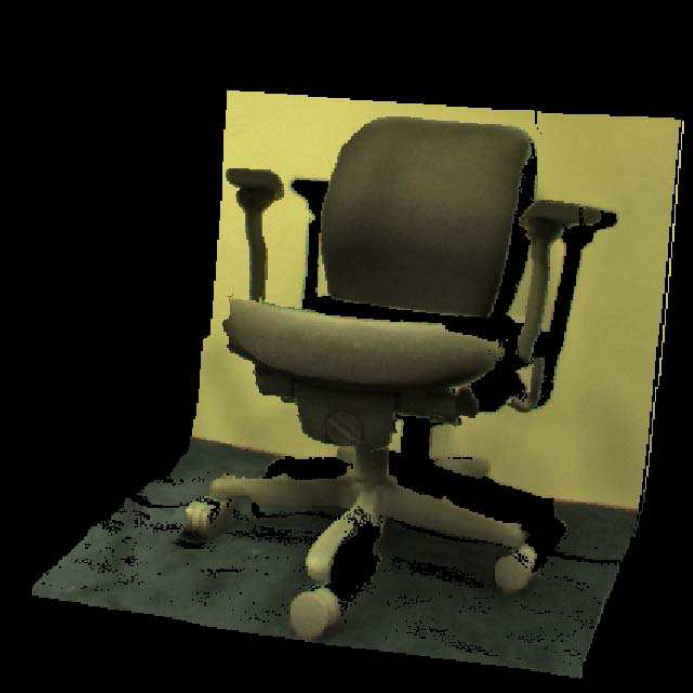
\includegraphics[height=5cm]{/home/bontius/workspace/cpp_projects/KinfuSuperRes/thesis/img/chair_gt.png}
	\end{minipage}
	\begin{minipage}[b]{0.49\linewidth}\centering
		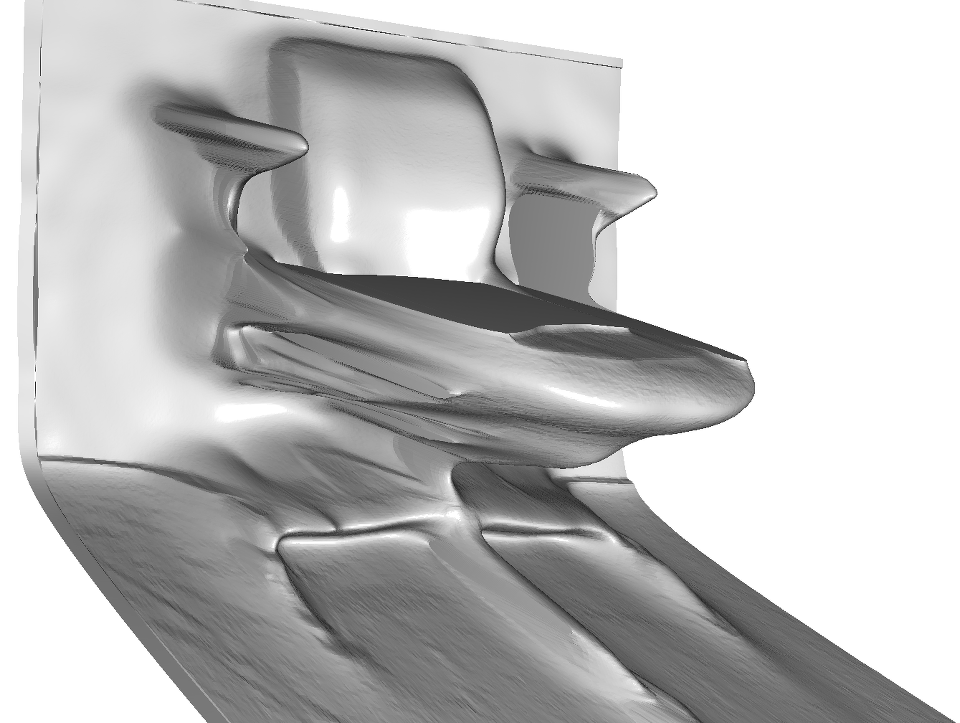
\includegraphics[height=5cm]{/home/bontius/workspace/cpp_projects/KinfuSuperRes/thesis/results/chair00.png}
	\end{minipage}
	\caption{"Chair" output by original paper (left) and by our implementation (right).}
	\label{fig:chair}
\end{figure}

\begin{figure}[h!]\centering
	\begin{minipage}[b]{0.49\linewidth}\centering
		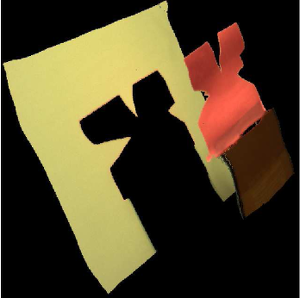
\includegraphics[height=5cm]{/home/bontius/workspace/cpp_projects/KinfuSuperRes/thesis/img/pink_gt.png}
	\end{minipage}
	\begin{minipage}[b]{0.49\linewidth}\centering
		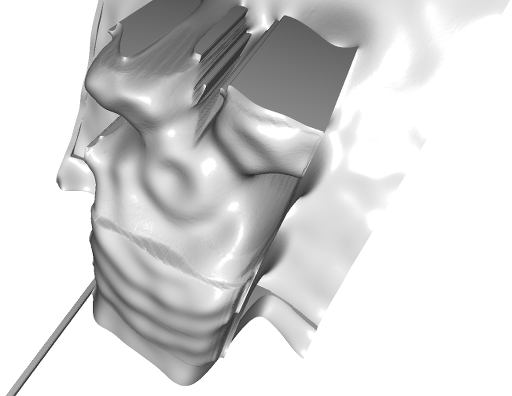
\includegraphics[height=5cm]{/home/bontius/workspace/cpp_projects/KinfuSuperRes/thesis/results/pink00.png}
	\end{minipage}
	\caption{"Pink" output by original paper (left) and by our implementation (right).}
	\label{fig:pink}
\end{figure}


%%% SECTION %%%
\section{Structure from motion} 
\label{sec:sfm}

\par Due to recent achievements of the fields multi-view stereo and structure from motion, the reconstruction capabilities of these methods were tested in the beginning of the project to decide, whether a sparse or dense 3D reconstruction algorithm is to be used. Recordings were created using the video recording function of a rather modern smart phone. The 1080p image stream was down sampled to 960 x 540, and the frame rate of the video was decreased using sub-sampling to 5 FPS. This data was input into both \citep{Photosynth} and \citep{vsfm}, state-of-the art sparse stereo reconstruction algorithms. In general, Microsoft Photosynth performed better with the reconstruction of these scenes. These tasks are otherwise considered to be hard for multi-view stereo due to transparency and the repetitive, feature-less characteristics of the recordings. Results are shown in \figref{fig:acerlit_1}, \figref{fig:acerlit_mesh}, \figref{fig:ob_1} and \figref{fig:ob_mesh}.

% acerlit image
\begin{figure}[h!]\centering
	\begin{minipage}[b]{0.4\linewidth}\centering
		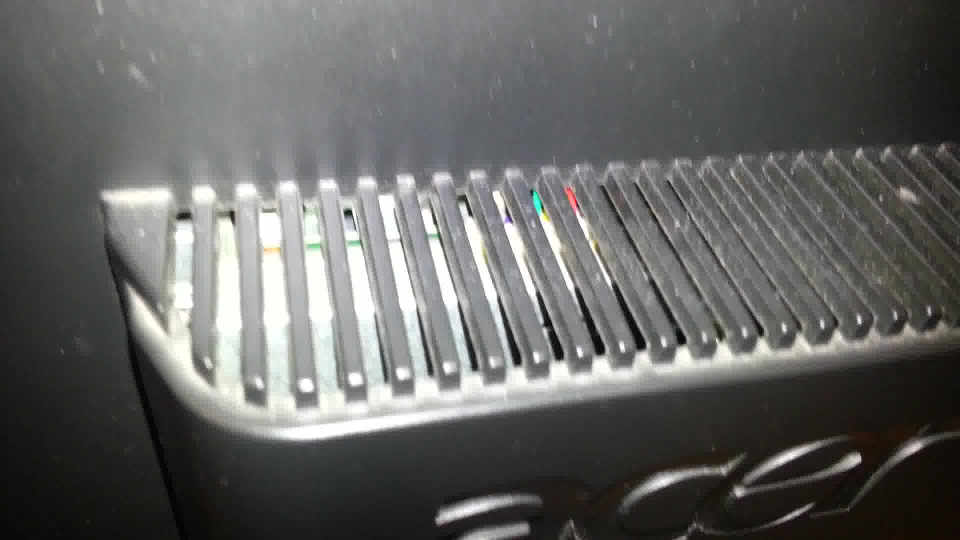
\includegraphics[height=5cm]{/home/bontius/workspace/cpp_projects/KinfuSuperRes/thesis/img/acer_lit00706.jpg}
		\caption{A frame of video of backside of a monitor.}
		\label{fig:acerlit_1}
	\end{minipage}
	\begin{minipage}[b]{0.49\linewidth}\centering
		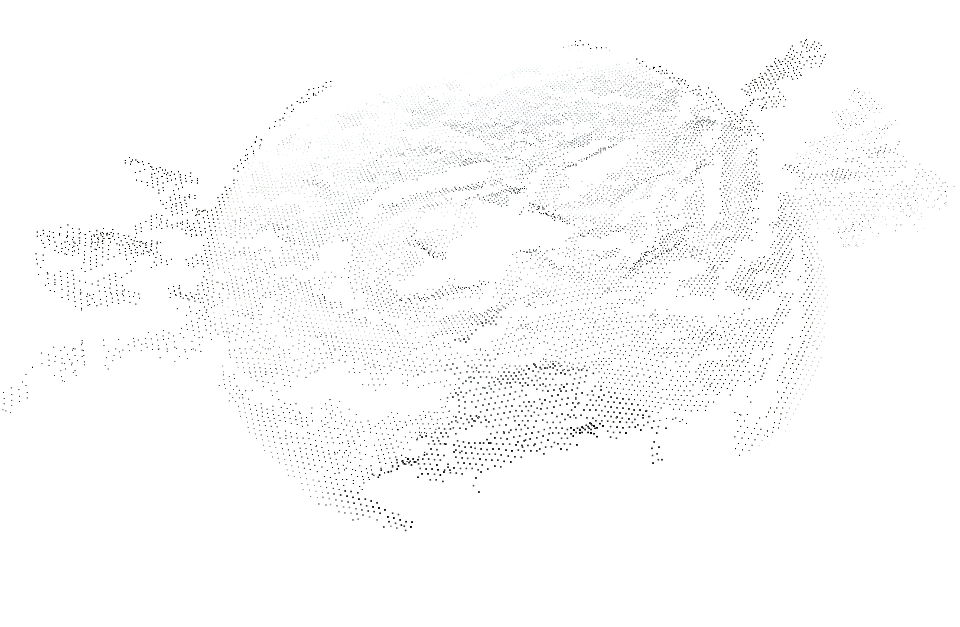
\includegraphics[height=5cm]{/home/bontius/workspace/cpp_projects/KinfuSuperRes/thesis/img/acer_lit01.png}
		\caption{Visual SFM 3D reconstruction of monitor. Almost no sense of 3D has been captured.}
		\label{fig:acerlit_mesh}
	\end{minipage}
\end{figure}

% oil bottle image
\begin{figure}[h!]\centering
	\begin{minipage}[b]{0.49\linewidth}\centering
		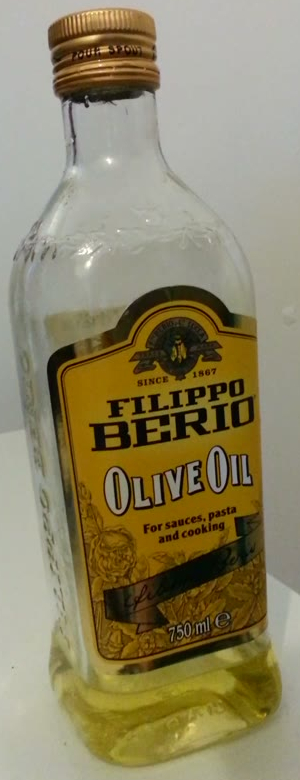
\includegraphics[height=5cm]{/home/bontius/workspace/cpp_projects/KinfuSuperRes/thesis/img/ob00003r2.jpg}
		\caption{A frame of video of oil bottle}
		\label{fig:ob_1}
	\end{minipage}
	\begin{minipage}[b]{0.49\linewidth}\centering
		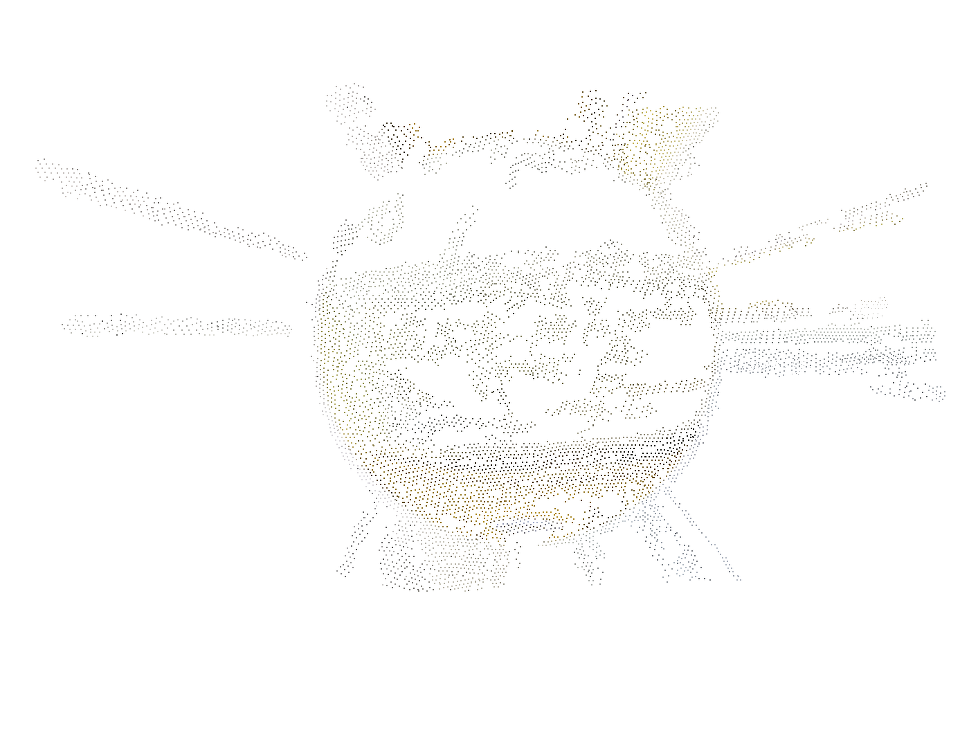
\includegraphics[height=5cm]{/home/bontius/workspace/cpp_projects/KinfuSuperRes/thesis/img/ob_mesh00.png}
		\caption{Visual SFM 3D reconstruction of oil bottle. Almost no sense of 3D has been captured.}
		\label{fig:ob_mesh}
	\end{minipage}
\end{figure}



\chapter{Discussion} 
\label{chp:discussion}

\section{Results}
\label{sec:discussion_results}

\par A thorough investigation has been performed in \chpref{chp:validation} to identify strengths and weaknesses of the designed system. Based on the evaluation we claim to have developed a proof-of-concept system that identifies major challenges arising during the solution of the targeted task. The initial hypothesis of existing discarded data can be regarded confirmed, since on all of the final output images in \secref{sec:results} we can see depth detail of granularity not observed in current 3D reconstruction algorithms. The level up to which the keyboard keys are  distinguishable in \figref{fig:keyboard2_192_final} is encouraging. However there is a very apparent problem of viewpoint dependency of the algorithm. In all resulting figures one can see, that the details are not put into the right depth, i.e. the keyboard keys are not elevated from the smooth surface, but partially sunk in. The problem becomes even more severe, when steep view-angles are observed as in \figref{fig:keyboard_192_final}. The fact, that the 3D depth data is mapped to the RGB image, and not the opposite can be attributed this effect. In future work, the possibilities of determining a decision logic, controlling whether the individual parts of the here shown up-sampled results should be integrated into the mesh. Another, possibly even more effective approach is to investigate, what conditions have to be fulfilled to be able to use the up-sampling algorithm from an ideal, normal directed viewpoint by taking the information conveyed in the new colour image into account through ray-casting it to the smooth mesh surface. Obviously the sparsity of the colour data would have to be one of the challenges to be targeted.

\par The decision about the possibility of rendering a virtual viewpoint and applying a newly acquired RGB image to enhance it's quality is not obvious. Although the calibration, smooth reconstruction and depth up-sampling steps of the pipeline have successfully been validated, the rendering and alignment of the new viewpoint has not. The problems are suspected to rely on two grounds. First, there are too many unknown factors for hold-one-out validation of the pose rendering. The calculation errors introduced by the changes of the intrinsic matrices due to aspect-ratio changing resolution transforms would have to be estimated using a more thorough approach. Second, the pose estimation accuracy of the Kinect Fusion algorithm is shown to be quite limited for the accurate needs of our pipeline. For example in \figref{fig:limit_kinfu_pose} one can see a reasonably well aligned depth and RGB image that come directly from the calibrated Kinect device. However, the virtual depth map and the RGB are misaligned, mostly along the y-axis. Since the aspect-ratio change due to resolution transformations happens along the x-axis, the Kinfu pose estimation is suspected to be the reason to the observed misalignment of the data. Additionally, the event-based, so called "triggered capture" nature of the middleware applied to the two fold difference in stream update speeds (15 FPS vs. 30 FPS) can also contribute to the pose estimation errors.

%
%\subsection{Dense or sparse reconstruction}
%
%\par An easy to operate, hand-held scanning device is used. The developed system will most likely use a smartphone with built in inertial measurement unit, gyroscope, magnetometer and GPS sensor. Alternatively a camera with mounted and calibrated motion and orientation sensors can be used. The performance of structured lighting devices as Microsoft Kinect \cite{Kinect} or Asus Xtion PRO \cite{XtionPro} will also be explored. Eventually a higher resolution device as Leap-motion's gesture recognition solution \cite{LeapMotion} will be evaluated. To ensure interchangeability of the sensors, and to get these systems to cooperate to the highest level possible, a well designed framework needs to be developed. The extensibility of the KinectFusion SDK will be tested once it get's released as part of the Windows 8 SDK as promised \cite{SDKKinectFusion}. Alternatives, as the implementation of a Kinect Fusion like functionality in the Point Cloud Library ("Kinfu") will also be tested \cite{KinFu}.
%\par The commercial accessibility of the used sensor setup has a slightly increased emphasis at this stage of the project. Low cost and out of the box operability would open the possibilities for crowd sourcing in follow-up projects, something that has been targeted by many other research labs as Microsoft (at Techfest 2013) or the University of Washington (Photocity, Pointcraft).
%
%/// The current sensor pose is simultaneously obtained by
%tracking the live depth frame relative to the global model using a
%coarse-to-fine iterative closest point (ICP) algorithm, which uses
%all of the observed depth data available. We demonstrate the advantages
%of tracking against the growing full surface model compared
%with frame-to-frame tracking, obtaining tracking and mapping results
%in constant time within room sized scenes with limited drift
%and high accuracy. We also show both qualitative and quantitative
%results relating to various aspects of our tracking and mapping system.
%Modelling of natural scenes, in real-time with only commodity
%sensor and GPU hardware, promises an exciting step forward
%in augmented reality (AR), in particular, it allows dense surfaces to
%be reconstructed in real-time, with a level of detail and robustness
%beyond any solution yet presented using passive computer vision.

\section{Limitations} 
\label{sec:limitations}

\par Based on the demonstrated results in \chpref{chp:validation} the strengths and weaknesses of the employed sub-systems can be assessed. The most important sub-systems evaluated are calibration, Kinect Fusion and depth up-sampling.
\par The calibration toolbox applied in this project is not the most advanced one. State of the art calibration treats range sensors differently by building a noise model before optimisation of the intrinsic parameters \citep{calibration_herrera}. The problem of IR to depth image misalignment is also overcome when estimating calibration using the depth images. More of these have to be acquired though, to provide enough data to the noise model estimation.
\par The Kinect Fusion implementation applied in this project provides a powerful method for smooth 3D reconstruction. It handles static mid-scale static scenes well, and degrades over dynamic scenes gracefully. State-of-the art improvements have targeted the limitations of the system used in this solution, such as limited work volume \citep{Whelan13iros}, averaging over scale space \citep{Fuhrmann:2011} and memory footprint \citep{keller13realtime}. The limitation faced in this project with the highest impact is the pose estimation accuracy. The applied ICP algorithm and it's static movement threshold did not yield suitable quality of the pose estimates. During reconstruction, sequences of frames were observed with larger displacement or more intensive viewangle changes where the pose estimation was a big problem. Around more static pose sequences in the recordings the pose estimates were observed to be okay. It is to be tested however, if these better alignments are of quality high enough to serve as input for any chosen depth up-sampling. State-of-the art visual odometry applies both streams to provide a better pose estimation \citep{Whelan13icra}. The possibility of applying machine learning methods and segmentation for more accurate calibration and pose estimation is also to be explored \citep{malisiewicz-iccv11}.

%%%% KINFU pose estimation %%%%
\begin{figure}[h!]\centering
	\begin{minipage}[b]{0.49\linewidth}
		\includegraphics[width=\textwidth]{/home/bontius/workspace_local/long640_20130829_1525_200_400/results/really_correct_intr/d138_blended.png}
		\caption{Aligned Kinect data. The estimated intrinsic and extrinsic relations of the camera are well suited for the purpose.}
	\end{minipage}
	\begin{minipage}[b]{0.49\linewidth}
		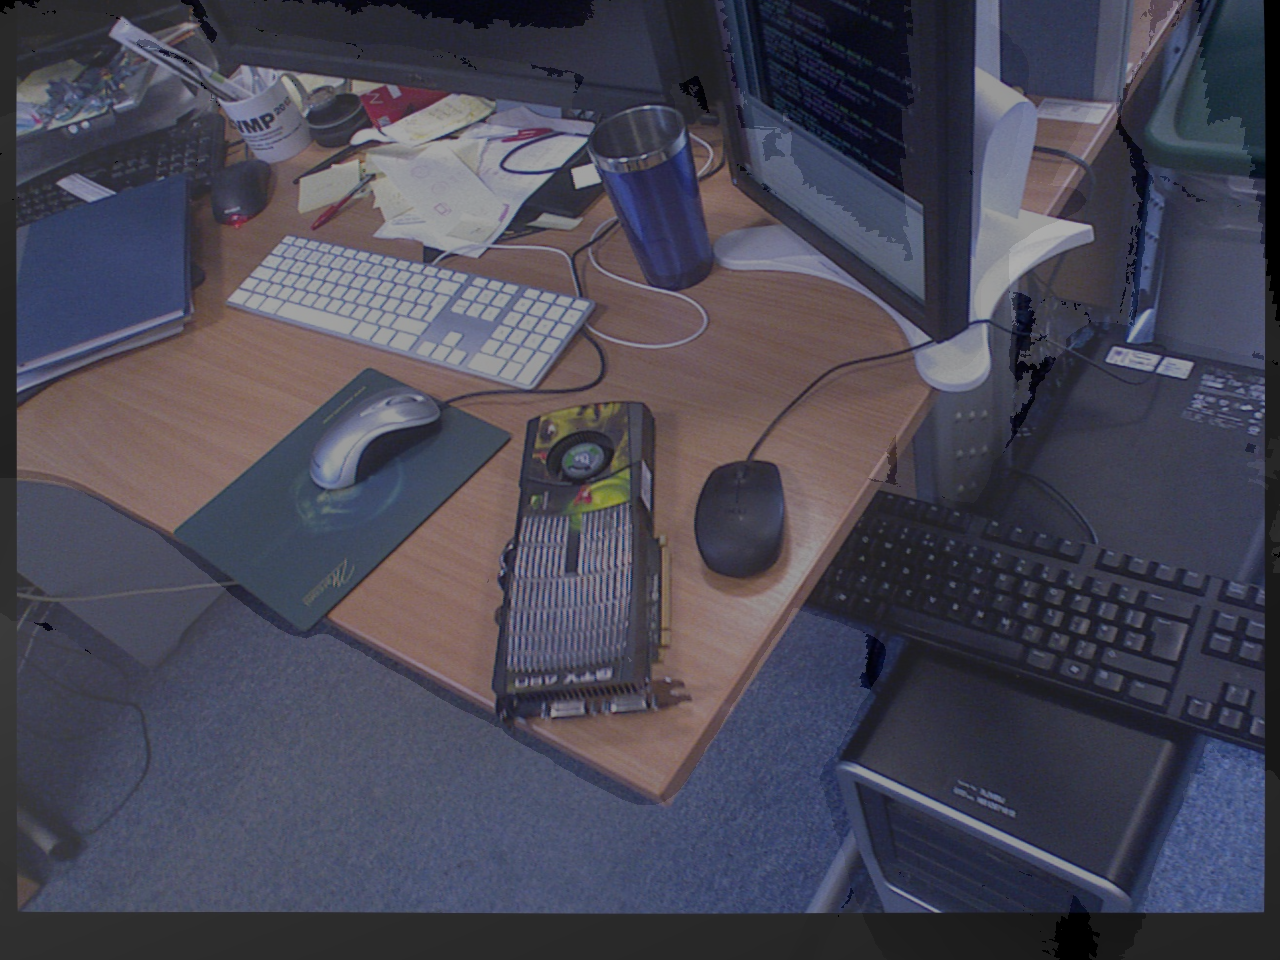
\includegraphics[width=\textwidth]{/home/bontius/workspace_local/long640_20130829_1525_200_400/results/really_correct_intr/kinfu_depth_138_blended.png}
		\caption{Misaligned KinFu pose estimation. The same parameters are used for the virtual viewpoint alignment.}
		\label{fig:limit_kinfu_pose}
	\end{minipage}
\end{figure}

This project has problems with the limitations introduced by the quality of the RGB camera as shown in \figref{fig:kinect_rgb_zoom}. This is only a practical limitation though, since the theoretical enables the application of high quality SLR cameras for refinement.

\begin{figure}[h!]\centering
        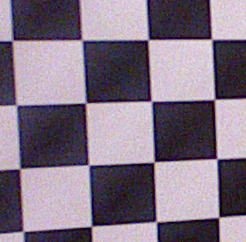
\includegraphics[width=\linewidth]{/home/bontius/workspace/cpp_projects/KinfuSuperRes/thesis/img/kinect_rgb_zoom.png}
        \caption{Kinect RGB image quality at 1280 x 1024 resolution}
        \label{fig:kinect_rgb_zoom}
\end{figure}

\par The strengths and weaknesses of the chosen and applied depth super-resolution technique introduced by \citep{cvpr-07-qingxiong-yang} have been well demonstrated in \secref{sec:results}. Its largely dependent on the alignment of its input images and is sensitive to non-geometric texturing. The latter has most noticeable impact observable around the sticker on the computer in \figref{fig:keyboard2_192_final}, or by the checker-board pattern in  \figref{fig:yang_checkerboard}. The method also requires fixed and hand-tuned parameters that allows limited adaptation to the data. The used parameters of the cross-bilateral filtering method were selected by creating a real-time visual feedback tool with the appropriate trackbars. This is not suitable for frame-by-frame usage, especially since the filtering is applied to the cost volumes and not the visual input frames. A limitation conveying large impact on our solution is the fact, that the filtering approach does not introduce new depth levels, as verified by experiment.
It is claimed by \citep{guided_filter}, that cross-bilateral filtering introduces an unwanted edge inversion effect, this effect is slightly observable in our output images. The direction of a more state-of-the art filtering technique using hybrid Euclidean-geodesic filters introduced by \citep{Gastal:2012} is to be explored.
    
\section{Future work}
\label{sec:future_work}

\par The experiences collected along the {\it Chapters \ref{chp:validation} and \ref{chp:discussion}} allow us to identify the most critical points of the algorithm needing improvement to continue with. The simulated and missing parts of the planned pipeline has to be solved. 

\par The calculation of the actual position of the virtual viewpoint of a new acquisition was simulated during this project. Bundle adjustment implemented in \citep{SnavelySS06} or \citep{vsfm} can be used to align the new RGB data with the available snapshots from the Kinect stream. The new sparse and stored dense reconstruction model can than be aligned by an ICP type algorithm, so that the estimated new camera pose can be transformed between the two coordinate systems.

\par In terms of innovation, the possibilities of determining a decision logic that controls whether the individual parts of the here shown, up-sampled results should be integrated into the mesh. The task of selection of the best viewpoint for a given 3D point and a set of existing camera poses points beyond greedy approaches of minimising distance and maximising normal angle. Ideas along the lines of \citep{Buehler:2001} and \citep{keller13realtime} have to be explored. Preceding work i.e. in \citep{Hoiem:2011} has been performed to handle the problems around occluded regions.
\par Another, possibly even more effective approach is to investigate, what conditions have to be fulfilled to be able to use the up-sampling algorithm from an ideal, normal directed viewpoint by taking the information conveyed in the new colour image into account through ray-casting it to the smooth mesh surface.

\par As identified earlier, intelligent alignment of the new recordings and the existing surface representation has to be performed in order to implement the simulated part of our pipeline. Ideas presented by \citep{Herrera:LearnedJointMRF} are to be investigated. The area of merging the up-sampled and selected depth details with the original model has to be solved using the knowledge of the geometry processing community.

\par Although the filtering technique applied provided promising results in terms of granularity of details. However the difficulties arising due to the characteristics of the approach and proposed solutions for earlier in this section might indicate, that better filtering approaches, or other up-sampling methods have to replace the currently used technique. \\

\par With the development of the domain of multi-view stereo the quality of surface reconstructions achieved might reach the point, where the basis of the solution can be exchanged for an even more commonly accessible recording device in form of a smartphone, or possibly a smartphone with a 3D camera. By moving the computation to the cloud, a  crowd sourcing based follow-up project can target the reconstruction of large scale, public areas. A solution highly suitable for the purposes of cultural heritage preservation.




%\section{System plan}
%	\begin{itemize}
%		\item Calibration
%			\begin{itemize}
%				\item Depth image based
%				\item IR image based
%				\item Undistort
%			\end{itemize}
%		\item Low resolution 3D reconstruction
%			\begin{itemize}
%				\item Multi View Stereo (VSFM, Bundler, Photosynth, etc.)
%				\item Kinect Fusion, PCL::Kinfu
%			\end{itemize}
%		\item Pose estimation of new input
%			\begin{itemize}
%				\item VSFM ( for RGB input )
%				\item ICP ( for RGB-D input )
%				\item Gyro+IMU (a noisy graph of acquired data)
%			\end{itemize}
%		\item Mesh subdivision (Linear, Butterfly, Catmull-Clark)
%		\item 2D projection
%			\begin{itemize}
% 				\item Raycasting using Octree
%				\item GLSL projection
%			\end{itemize}
%		\item Yang filtering
%			\begin{itemize}
%				\item Iterative Cross Bilateral filtering
%				\item Subpixel accurracy
%			\end{itemize}
%		\item Mesh enhancement by backprojection
%	\end{itemize}
%	
%\section{System design}
%	\begin{itemize}
%		\item Implementation details and takeaway experience of "System plan" elements
%		\item Merge into previous?
%	\end{itemize}
%	
%\section{Evaluation}
%	\begin{itemize}
% 	\item Experiments
%		\begin{itemize}
%			\item Calibration
%				\begin{itemize}
%					\item Kinect built in calibration
%					\item Bogouet calibration with and without lens distortion (PARAMETERS explained)
%					\item Undistort effectivity (project undistorted depth map to 3D)
%				\end{itemize}
%				
%			\item Filtering
%				\begin{itemize}
%					\item CrossBilateral filter vs. Bilateral
%					\item Yang vs. CrossBilateral (PARAMETERS explained)
%					\item Trilateral, Guided, Pixel Weighted Average Strategy (Garcia et al,ImProc, 2010) - {\bf IF there's time}
%				\end{itemize}
%			\item Kinect fusion related
%			\begin{itemize}
%				\item Kinfu vs. Kinfu w/ filtering turned OFF
%				\item Kinfu voxel grid resolution ($386^3$,$512^3$,$640^3$)
%				\item Kinfu + Yang( original kinect depth frames )
%				\item Kinfu + Yang( "arbitrary pose" )
%			\end{itemize}
%		\end{itemize}
%	\item Existing libraries used
%	\item Data capturing details
%	\item No existing datasets compared (no time)
%
%	\end{itemize}
%
%\section{Results}
%\begin{itemize}
%	\item Upsampling with original depth frames
%	\item Upsampling with simulated "arbitrary pose"
%
%	\item original yang images
%	\item subpixel refinement
%	
%	\item So, Yang is is not suitable for this resolution, it only could improve, when the input was much noisier
%	\item Different approaches can be plugged in to this framework to enhance depth
%\end{itemize}
%\section{Conclusions, Future work}
%	\begin{itemize}
%		\item 3D reconstruction improvements
%			\begin{itemize}
%				\item Improve on smoothing effect of voxel grid weights
%				\item Pose estimation improvements
%			\end{itemize}
%		\item RGB high-resolution capture, vsfm pose estimation 
%		\item Enhancement by best pose selection from input image collection for given pixel/region
%	\end{itemize}
 
%\bibliographystyle{plainnat}
\bibliography{litrev}
	
\end{document}


% \lstset{style=customcpp}
%\begin{lstlisting}
%__device__ float yangRangeDist( float4 a, float4 b, float sigma )
%{
%    float mod = ( fabs(b.x - a.x) +
%                  fabs(b.y - a.y) +
%                  fabs(b.z - a.z)  ) / 3.f;
%    return __expf(-mod / sigma);
%}
%template <typename T>
%__global__ void
%d_cross_bilateral_filterF( T *dOut, int w, int h, size_t outPitch,
%                           float range_sigma, int r, bool onlyZeros = false )
%{
%    int x = blockIdx.x*blockDim.x + threadIdx.x;
%    int y = blockIdx.y*blockDim.y + threadIdx.y;
%
%    if (x >= w || y >= h) return;
%
%    float sum = 0.f, factor = 0.f, t = 0.f;
%    float4 guideCenter = tex2D( guideTex, x, y );
%    T      centerPix   = fetchTexture<T>( x, y );
%
%    // check for early exit
%    if ( onlyZeros && (centerPix != 0.f) )
%    {
%        dOut[y * outPitch + x] = centerPix;
%        return;
%    }
%
%    // estimate cost volume
%    for ( int i = -r; i <= r; ++i )
%    {
%        for ( int j = -r; j <= r; ++j )
%        {
%            // read depth
%            T curPix = fetchTexture<T>( x+j, y+i );
%            // skip, if no data
%            if ( onlyZeros && curPix == 0.f )
%                continue;
%            // read rgb
%            float4 guidePix = tex2D( guideTex, x + j, y + i );
%            // estimate weights
%            factor = cGaussian[i + r] * cGaussian[j + r] *
%                     yangRangeDist( guidePix, guideCenter, range_sigma );
%            // accumulate
%            t   += factor * curPix;
%            sum += factor;
%        }
%    }
%    if ( sum > 0.f )
%        dOut[y * outPitch + x] = t / sum;
%    else
%        dOut[y * outPitch + x] = centerPix;
%}
%
%\end{lstlisting}